\PassOptionsToPackage{table, svgnames, dvipsnames}{xcolor}

\documentclass[a4paper,12pt]{article}
\usepackage[utf8]{inputenc}
\usepackage[a4paper,margin=1in]{geometry}
\usepackage{pdflscape}
\usepackage{setspace}
\usepackage{graphicx} % Required for inserting images
\usepackage{amsmath}
\usepackage{authblk}
\usepackage{caption}
\usepackage{subcaption}
\usepackage{ulem}
\usepackage{multirow}
\usepackage{hyperref}
\usepackage{tikz}
\usepackage{xcolor}
\usepackage{caption}
\usepackage{geometry}
\geometry{a4paper,margin=1in}
\usetikzlibrary{patterns}
\usepackage{pgfplots}
\usepgfplotslibrary{groupplots}
\pgfplotsset{compat=1.18}
\usetikzlibrary{positioning, shapes, arrows.meta}
\usepackage{adjustbox}
\usepackage[margin=1in]{geometry}
\usepackage{setspace}

%REFERENCES
\usepackage{natbib}
\bibliographystyle{apalike}

%LONGTABLE
\usepackage{xcolor}
\usepackage{longtable}


\usepackage{adjustbox, rotating, threeparttable}
\usepackage{makecell, cellspace, caption}
\usepackage{array}
\usepackage{booktabs}

\usepackage{pifont} % シンボルを使うために必要なパッケージ



%脚注
\usepackage{footmisc}


\begin{document}

\title{Does the Gender Income Gap Expand Due to Natural Disasters? Evidence from the Great East Japan Earthquake}

\author{Tomoto Masuda}


\date{\today}

\maketitle

\begin{center}
    \textbf{Abstract}
\end{center}

\noindent
This study examines the effects of the Great East Japan Earthquake of March 11, 2011, which led to a catastrophic tsunami and triggered a nuclear incident at Fukushima, on the gender income gap in Fukushima Prefecture. Employing an event study approach alongside a difference-in-differences (DID) methodology, this study examines the disaster's influence on gender-based economic dynamics. Drawing on extensive prefectural economic statistical data and individual socio-economic attributes from sources such as the Japan General Social Survey (JGSS), the Open Survey Data Japan Household Panel Survey on Consumer Preferences and Satisfaction (JHPS-CPS), the Population Census, and the Housing and Land Survey, this study assesses the long-term effects of the disaster on the gender income gap. The results indicate that, in contrast to the immediate aftermath, the long-term impacts have attenuated significantly. This convergence can be attributed to multiple factors, including employment policies and the time lag between their implementation and observable effects, the economically rational adaptations of households in response to disruptions in community structures, and the possibility that the destruction of communities by the disaster also disrupted traditional gender norms and local gift economies, pushing women into the labor market.


\newpage

\tableofcontents


\clearpage
\section{Introduction}
\label{sec1}


The impact of large-scale natural disasters on Gender Employment Gaps remains insufficiently understood, despite both being crucial policy concerns. Previous studies present mixed findings on the impact of natural disasters on gender inequality, with some research indicating that such disasters exacerbate gender gaps while others suggest a narrowing of these disparities. The Great East Japan Earthquake presented a unique opportunity to examine the dynamics of labor market responses to significant external shocks. This study focuses on Fukushima Prefecture, an area profoundly affected by both the earthquake and subsequent nuclear incident, to analyze the short-term and long-term impacts on the gender employment gap.

Firstly, this study contributes to the literature by synthesizing two seemingly contradictory theoretical frameworks concerning disasters and gender disparities in labor markets. On one hand, development economics posits that shock-coping strategies may attenuate gender gaps through increased labor supply. On the other hand, the Risk Adjustment Hypothesis suggests that shocks disproportionately exclude women from the workforce. By reconciling these ostensibly divergent perspectives, this study offers a nuanced understanding of gender-based labor outcomes in the context of disasters.

Secondly, the model incorporates the concepts of economic shocks and adaptation mechanisms. The immediate aftermath of the disaster likely triggered rapid changes in employment patterns. However, over time, households develop adaptation strategies, including adjustments in labor supply preferences and reallocation of household labor responsibilities.

Lastly, the model considers the impact of community structure changes on household decision-making. The earthquake and its aftermath significantly disrupted local infrastructure and social networks, potentially altering the context in which households make employment decisions. Additionally, the disruption of traditional gender norms and local gift economies may have compelled women to enter the labor market. This study posits that long-term community rebuilding efforts can influence labor market dynamics and potentially reshape gender roles within households and the broader community.

By integrating these three elements - household decision-making, economic shocks and adaptation, and community disruption - the theoretical model provides a comprehensive framework for understanding the complex interplay of factors affecting the gender employment gap in the aftermath of a natural disaster.

\section{Background}
\label{sec2}

\subsection{The Great East Japan Earthquake }
\label{sec5.1}

 In Japan, the triple disaster of the Great East Japan Earthquake, the ensuing tsunami, and the Fukushima Daiichi nuclear crisis will have enduring implications on public perceptions of both local and national government authorities, as well as specialists in relevant fields. Furthermore, this disaster has profoundly reshaped attitudes towards nuclear energy, highlighting its risks and prompting widespread reconsideration of its role in Japan's energy strategy.


The Great East Japan Earthquake of March 2011 resulted in a tripartite catastrophe, comprising a magnitude 9.0 earthquake, a devastating tsunami, and a nuclear accident at the Fukushima Dai-ichi Nuclear Power plant. This disaster precipitated a severe humanitarian crisis, causing extensive damage particularly in the Iwate, Miyagi, and Fukushima prefectures in northeast Japan. According to the National Police Agency, 15,900 people lost their lives and 2,523 people remain unaccounted for, primarily as a result of the massive tsunami that struck the eastern coast of Japan. The affected prefectures account for 99.6\% of total fatalities and 99.8\% of total missing persons. In addition, a total of 3,784 fatalities and casualties were recognized as disaster-related deaths in Japan due to the exacerbation of chronic illnesses or suicide during evacuation. Approximately 90\% of fatalities were attributed to drowning. Table 1 presents a summary of the damages in the affected prefectures. The map below indicates the epicenter of the earthquake.

\begin{flushleft}
\begin{table}[h!]
  \caption{Direct Impact Overview in the Disaster-Stricken Prefectures}\label{table:disaster_situation}
  \begin{minipage}[c]{0.4\textwidth}
    \includegraphics[width=\textwidth,height=1.10\textwidth]{epicenter.jpeg}
  \end{minipage}
  \begin{minipage}[c]{0.48\textwidth}
    \raggedright
    \scalebox{0.8}{
    \begin{tabular}{|c|c|c|c|}
    \hline
    & \multicolumn{1}{c|}{Iwate} & \multicolumn{1}{c|}{Miyagi} & \multicolumn{1}{c|}{Fukushima} \\
    \hline
    Population & 1,330,147 & 2,348,165 & 2,029,064 \\
    Deceased & 4,675 & 9,544 & 1,614 \\
    Missing & 1,110 & 1,213 & 196 \\
    Fully destroyed houses & 20,185 & 83,932 & 20,136 \\
    Partially destroyed houses & 4,562 & 138,721 & 65,093 \\
    \hline
    \end{tabular}
    }
  \end{minipage}
\end{table}
\end{flushleft}

Fukushima Prefecture experienced a compound disaster involving both the tsunami triggered by the earthquake and the subsequent nuclear accident. The nuclear incident, in particular, necessitated large-scale evacuations, significantly disrupting local communities and labor markets. This unprecedented situation provides a unique context for examining the long-term socioeconomic impacts of compound disasters.

\subsection{Gender Dimensions of Disaster Risk and Resilience}
\label{sec5.1}

According to the latest 2024 Global Gender Gap Report by the World Economic Forum (WEF), Japan ranks 118th out of 146 countries, placing it at the bottom among the G7 nations. Particularly, its rankings in the "Economic" and "Political" domains are notably low, with the "Economic" ranking being 120th out of 146 countries. Japan continues to exhibit substantial gender disparities in the economic sector, with the elimination of wage gaps remaining a significant challenge.

The ‘Act on Promotion of Women’s Participation and Advancement in the Workplace’ enacted in April 2016 has led to the development of an environment conducive to working women of child-rearing generations, with initiatives such as the introduction of a reduced working hours system, restrictions on overtime work, and the establishment of childcare facilities within companies. The Gender Equality Bureau of the Cabinet Office has also focused on supporting women in disaster-affected areas by addressing reconstruction efforts from a gender perspective, catering to the specific needs of women, and addressing child-rearing requirements.


\section{Literature review}
\label{sec3}

Nearly every empirical study of natural disasters finds short-term declines in either income or employment especially for groups vulnerable to disasters, such as primary industry workers, non-regular workers, women, and the elderly. 

%The exact magnitude of such effects on output is nevertheless widely debated. Some authors argue that earthquakes (and natural disasters in general) have significant negative effects on economic growth (Barro and i Martin 2003, Raddatz 2009). Recent work also notes potential spillovers propagating throughout the economy via trade linkages and supply chains (The et al. 2011, Ruta et al. 2021). Others, however, find mild or even positive effects on growth (Albala-Bertrand 1993, Barone and Mocetti 2014, Caselli and Malhotra 2004, Loayza et al. 2012, Porcelli and Trezzi 2019, Skidmore and Toya 2002).


\subsection{Literature on a risk adjustment hypothesis}
\label{sec5.1}


The risk adjustment hypothesis in labor economics suggests that during economic shocks or natural disasters, women are more vulnerable to labor market exclusion and face higher risks of deteriorating work conditions or unemployment compared to men. 


The non-regular workers, often function as 'adjustment valves,' absorbing economic shocks. These groups are disproportionately affected, serving as mechanisms to mitigate broader economic impacts. This framework illuminates the gender-based disparities in employment stability and the uneven distribution of economic resilience across worker categories during crises. For instance, \citet{Kim2014ARetention} examines the economic impact of the 2010 earthquake in Haiti, focusing on changes in household composition and employment retention. Authors found that the earthquake caused a significant reduction in employment rates, from 52.6\% prior to the earthquake to 28.6\% five months post-event. Gender disparities were evident, with only 34.2\% of women retaining their employment compared to 55.6\% of men. 


\citet{Groger2016InternalTyphoon} identified significant income shocks from Typhoon Ketsana in Vietnam using satellite imagery and household panel data. They found that affected households experienced a 10\% income decline, primarily due to crop losses. The study revealed that internal labor migration to urban areas served as a crucial coping mechanism, with households leveraging both existing migrant networks and sending new migrants to mitigate economic impacts through remittances.

\subsection{Literature on a shock coping strategy}
\label{sec5.1}

On the other hand, development economics posits that households increase their labor supply as a shock-coping strategy in response to natural disasters. This phenomenon is part of the broader concept of non-market insurance mechanisms, which play a crucial role in post-disaster recovery and risk management. Several studies demonstrate that labor markets can function as an ex-post risk coping mechanism following natural disasters. Studies have shown that households, particularly women, increase their labor supply as a risk mitigation strategy. 

 \citet{Porcelli2019TheItaly} conducted a counterfactual analysis using a balanced panel of 95 Italian provinces, examining the impact of 22 earthquakes on output and employment from 1986 to 2011. Their study, which compared affected provinces with similar neighboring provinces, revealed that the economic contraction following seismic events was generally minimal. In some instances, the net effect on output and employment was positive, as reconstruction activities outweighed the destruction of physical capital.

\citet{Deryugina2018TheReturns} analyzed Hurricane Katrina's long-term economic impact on New Orleans residents. While victims initially experienced significant income losses and reduced employment, within a few years their incomes and employment rates not only recovered but surpassed those of a control group.


\citet{Canessa2021WomensShocks} demonstrate that natural disasters can increase women's labor force participation. Using georeferenced longitudinal household panel data and a difference-in-differences approach, they found that severe flooding in Bangladesh led to a 13 percentage point increase in women's employment probability. This effect was particularly pronounced among lower-income households and women previously engaged in unpaid family farm work. The study reveals that women entered the workforce to mitigate income losses, especially in agriculture-dependent households. Additionally, women who transitioned to paid work outside family farms experienced increased household decision-making power, supporting theories of economic empowerment through independent income.

This study tries to fill gaps in the still sparse literature on the impact of natural disasters on gender disparities by differentiating between short-term and long-term effects, addressing the contradictory findings of existing research that suggests either an exacerbation or a reduction of gender gaps.


\section{Pre-Disaster Labor Market Structure and Post-Disaster Impact}
\label{sec4}

This section examines the structure of Fukushima Prefecture's labor market before the disaster, using data from the 2010 Population Census to overview occupations and employment types by gender. It then explores the economic impact of the disaster.


\subsection{Employment sector and type in Fukushima pref}
\label{sec4.1}

Examining the proportion of employed persons aged 15 and over by industry and sex in Fukushima Prefecture, manufacturing accounts for the highest share among males at 23.5\%, followed by construction at 12.9\%. In contrast, construction represents only 2.6\% of female employment (Figure~\ref{fig:fukushima_employment}).

%福島県の男女別15歳以上就業者について、産業別の割合をみると、男性は「製造業」が23.5%と最も高く、次いで「建設業」が12.9%となっている。女性では建設業はわずか2.6%に留まる(Figure 1)。

%%%%%%%%%%%%%%%%%%%%%%%%%%%%%%%%%%%%%%%%%%%%%


\begin{figure}[!htbp]
\centering 
\hspace*{-0.2cm} % Position of the graph
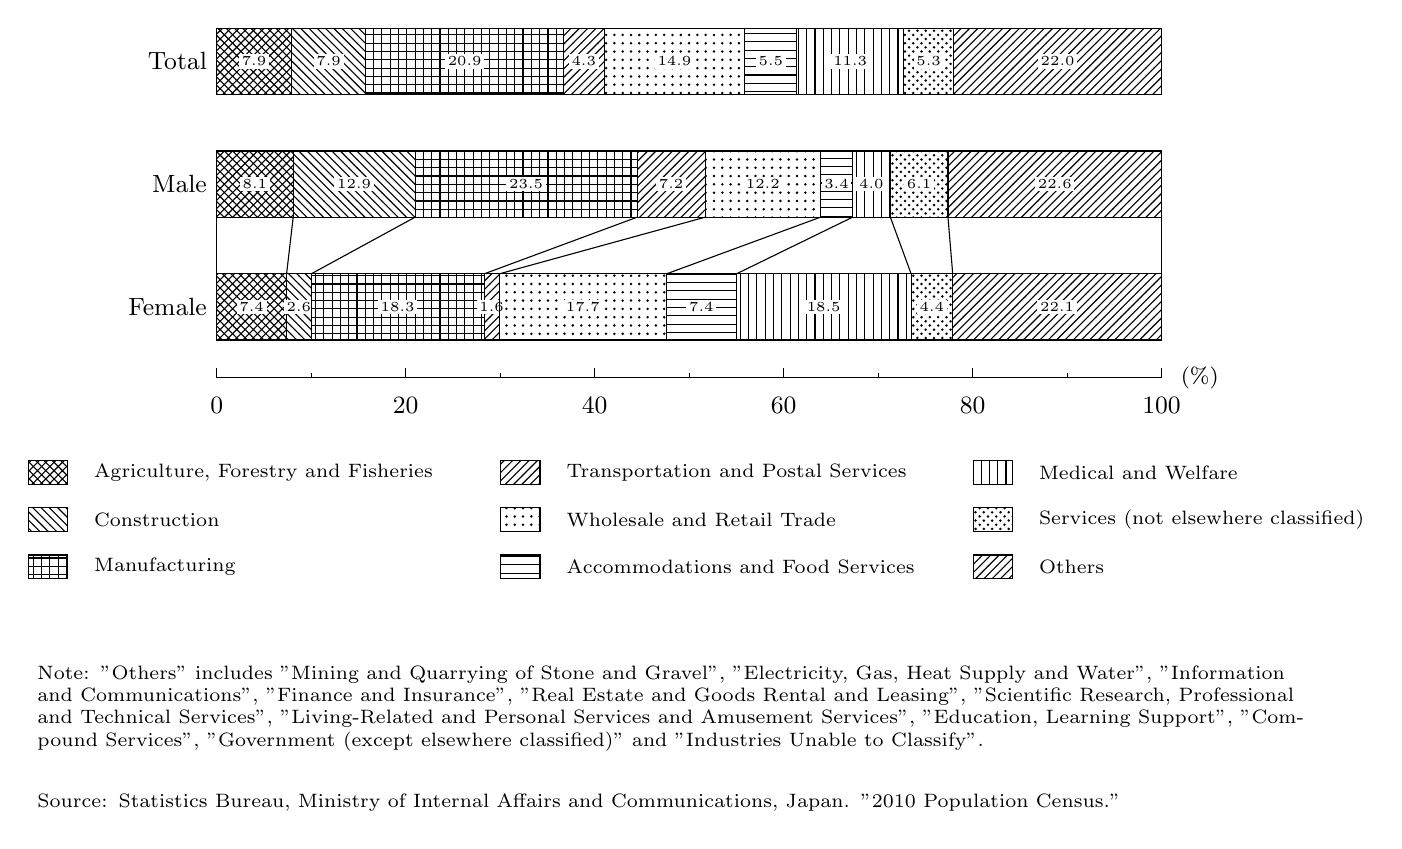
\begin{tikzpicture}[scale=1.20]
\definecolor{color1}{RGB}{200,200,200} 
\definecolor{color2}{RGB}{150,150,150} 
\definecolor{color3}{RGB}{100,100,100}
\definecolor{color4}{RGB}{250,200,200}
\definecolor{color5}{RGB}{200,150,150}
\definecolor{color6}{RGB}{150,100,100}
\definecolor{color7}{RGB}{100,50,50}
\definecolor{color8}{RGB}{50,0,0}
\definecolor{color9}{RGB}{0,0,0}

% Total bar
\draw[fill=color1, pattern=crosshatch] (2,9) rectangle (2.79,9.7) node[pos=0.5, fill=white, inner sep=1pt] {\tiny 7.9};
\draw[fill=color2, pattern=north west lines] (2.79,9) rectangle (3.58,9.7) node[pos=0.5, fill=white, inner sep=1pt] {\tiny 7.9};
\draw[fill=color3, pattern=grid] (3.58,9) rectangle (5.67,9.7) node[pos=0.5, fill=white, inner sep=1pt] {\tiny 20.9};
\draw[fill=color4, pattern=north east lines] (5.67,9) rectangle (6.10,9.7) node[pos=0.5, fill=white, inner sep=1pt] {\tiny 4.3}; 
\draw[fill=color5, pattern=dots] (6.10,9) rectangle (7.59,9.7) node[pos=0.5, fill=white, inner sep=1pt] {\tiny 14.9}; 
\draw[fill=color6, pattern=horizontal lines] (7.59,9) rectangle (8.14,9.7) node[pos=0.5, fill=white, inner sep=1pt] {\tiny 5.5};
\draw[fill=color7, pattern=vertical lines] (8.14,9) rectangle (9.27,9.7) node[pos=0.5, fill=white, inner sep=1pt] {\tiny 11.3};
\draw[fill=color8, pattern=crosshatch dots] (9.27,9) rectangle (9.80,9.7) node[pos=0.5, fill=white, inner sep=1pt] {\tiny 5.3};
\draw[fill=color9, pattern=north east lines] (9.80,9) rectangle (12,9.7) node[pos=0.5, fill=white, inner sep=1pt] {\tiny 22.0}; 

% Male bar
\draw[fill=color1, pattern=crosshatch] (2,7.7) rectangle (2.81,8.4) node[pos=0.5, fill=white, inner sep=1pt] {\tiny 8.1};
\draw[fill=color2, pattern=north west lines] (2.81,7.7) rectangle (4.10,8.4) node[pos=0.5, fill=white, inner sep=1pt] {\tiny 12.9};
\draw[fill=color3, pattern=grid] (4.10,7.7) rectangle (6.45,8.4) node[pos=0.5, fill=white, inner sep=1pt] {\tiny 23.5};
\draw[fill=color4, pattern=north east lines] (6.45,7.7) rectangle (7.17,8.4) node[pos=0.5, fill=white, inner sep=1pt] {\tiny 7.2}; 
\draw[fill=color5, pattern=dots] (7.17,7.7) rectangle (8.39,8.4) node[pos=0.5, fill=white, inner sep=1pt] {\tiny 12.2}; 
\draw[fill=color6, pattern=horizontal lines] (8.39,7.7) rectangle (8.73,8.4) node[pos=0.5, fill=white, inner sep=1pt] {\tiny 3.4};
\draw[fill=color7, pattern=vertical lines] (8.73,7.7) rectangle (9.13,8.4) node[pos=0.5, fill=white, inner sep=1pt] {\tiny 4.0};
\draw[fill=color8, pattern=crosshatch dots] (9.13,7.7) rectangle (9.74,8.4) node[pos=0.5, fill=white, inner sep=1pt] {\tiny 6.1};
\draw[fill=color9, pattern=north east lines] (9.74,7.7) rectangle (12,8.4) node[pos=0.5, fill=white, inner sep=1pt] {\tiny 22.6};

% Female bar
\draw[fill=color1, pattern=crosshatch] (2,6.4) rectangle (2.74,7.1) node[pos=0.5, fill=white, inner sep=1pt] {\tiny 7.4};
\draw[fill=color2, pattern=north west lines] (2.74,6.4) rectangle (3.00,7.1) node[pos=0.5, fill=white, inner sep=1pt] {\tiny 2.6};
\draw[fill=color3, pattern=grid] (3.00,6.4) rectangle (4.83,7.1) node[pos=0.5, fill=white, inner sep=1pt] {\tiny 18.3};
\draw[fill=color4, pattern=north east lines] (4.83,6.4) rectangle (4.99,7.1) node[pos=0.5, fill=white, inner sep=1pt] {\tiny 1.6}; 
\draw[fill=color5, pattern=dots] (4.99,6.4) rectangle (6.76,7.1) node[pos=0.5, fill=white, inner sep=1pt] {\tiny 17.7}; 
\draw[fill=color6, pattern=horizontal lines] (6.76,6.4) rectangle (7.50,7.1) node[pos=0.5, fill=white, inner sep=1pt] {\tiny 7.4};
\draw[fill=color7, pattern=vertical lines] (7.50,6.4) rectangle (9.35,7.1) node[pos=0.5, fill=white, inner sep=1pt] {\tiny 18.5};
\draw[fill=color8, pattern=crosshatch dots] (9.35,6.4) rectangle (9.79,7.1) node[pos=0.5, fill=white, inner sep=1pt] {\tiny 4.4};
\draw[fill=color9, pattern=north east lines] (9.79,6.4) rectangle (12,7.1) node[pos=0.5, fill=white, inner sep=1pt] {\tiny 22.1}; 

% Male to Female guidelines
\draw[thin] (2,7.7) -- (2,7.1);
\draw[thin] (2.81,7.7) -- (2.74,7.1);
\draw[thin] (4.10,7.7) -- (3.00,7.1);
\draw[thin] (6.45,7.7) -- (4.83,7.1);
\draw[thin] (7.17,7.7) -- (4.99,7.1);
\draw[thin] (8.39,7.7) -- (6.76,7.1);
\draw[thin] (8.73,7.7) -- (7.50,7.1);
\draw[thin] (9.13,7.7) -- (9.35,7.1);
\draw[thin] (9.74,7.7) -- (9.79,7.1);
\draw[thin] (12,7.7) -- (12,7.1);

% Labels
\node[anchor=east] at (2,9.35) {\small Total};
\node[anchor=east] at (2,8.05) {\small Male};
\node[anchor=east] at (2,6.75) {\small Female};

% X-axis
\draw (2,6) -- (12,6);
\foreach \x in {0,20,40,60,80,100}
    \draw (2+\x/10,6) -- (2+\x/10,6.1) node[anchor=north] at (2+\x/10,5.9) {\small \x};
\foreach \x in {10,30,50,70,90}
    \draw (2+\x/10,6) -- (2+\x/10,6.05);
\node[anchor=west, font=\footnotesize] at (12.1,6) {(\%)};

% Legend
\node[anchor=west, fill=color1, pattern=crosshatch, minimum width=0.5cm, minimum height=0.3cm, draw] at (0,5) {};
\node[anchor=west] at (0.6,5) {\scriptsize Agriculture, Forestry and Fisheries};
\node[anchor=west, fill=color2, pattern=north west lines, minimum width=0.5cm, minimum height=0.3cm, draw] at (0,4.5) {};
\node[anchor=west] at (0.6,4.5) {\scriptsize Construction};
\node[anchor=west, fill=color3, pattern=grid, minimum width=0.5cm, minimum height=0.3cm, draw] at (0,4) {};
\node[anchor=west] at (0.6,4) {\scriptsize Manufacturing};
\node[anchor=west, fill=color4, pattern=north east lines, minimum width=0.5cm, minimum height=0.3cm, draw] at (5,5) {};
\node[anchor=west] at (5.6,5) {\scriptsize Transportation and Postal Services};
\node[anchor=west, fill=color5, pattern=dots, minimum width=0.5cm, minimum height=0.3cm, draw] at (5,4.5) {};
\node[anchor=west] at (5.6,4.5) {\scriptsize Wholesale and Retail Trade};
\node[anchor=west, fill=color6, pattern=horizontal lines, minimum width=0.5cm, minimum height=0.3cm, draw] at (5,4) {};
\node[anchor=west] at (5.6,4) {\scriptsize Accommodations and Food Services};
\node[anchor=west, fill=color7, pattern=vertical lines, minimum width=0.5cm, minimum height=0.3cm, draw] at (10,5) {};
\node[anchor=west] at (10.6,5) {\scriptsize Medical and Welfare};
\node[anchor=west, fill=color8, pattern=crosshatch dots, minimum width=0.5cm, minimum height=0.3cm, draw] at (10,4.5) {};
\node[anchor=west] at (10.6,4.5) {\scriptsize Services (not elsewhere classified)};
\node[anchor=west, fill=color9, pattern=north east lines, minimum width=0.5cm, minimum height=0.3cm, draw] at (10,4) {};
\node[anchor=west] at (10.6,4) {\scriptsize Others};

% Annotation and Source
\node[text width=16.3cm, anchor=west, font=\scriptsize, align=left] at (0,2.5) {Note: "Others" includes "Mining and Quarrying of Stone and Gravel", "Electricity, Gas, Heat Supply and Water", "Information and Communications", "Finance and Insurance", "Real Estate and Goods Rental and Leasing", "Scientific Research, Professional and Technical Services", "Living-Related and Personal Services and Amusement Services", "Education, Learning Support", "Compound Services", "Government (except elsewhere classified)" and "Industries Unable to Classify".};

\node[text width=16.3cm, anchor=west, font=\scriptsize, align=left] at (0,1.5) {Source: Statistics Bureau, Ministry of Internal Affairs and Communications, Japan. "2010 Population Census."};

\end{tikzpicture} 
\caption{Proportion of Employed Persons Aged 15 and Over by Industry and Sex - Fukushima Pref. (2010)} 
\label{fig:fukushima_employment}

\end{figure}


%%%%%%%%%%%%%%%%%%%%%%%%%%%%%%%%%%%%%%%%%%%%%

%福島県の15歳以上就業者について、産業別の労働者割合を年齢層別にみると、津波や原子力発電所の事故災害の影響をもっとも受けた「農林漁業従事者」では男女共に65歳以上の割合が最も高い産業である。 一方で、復興需要の恩恵をもっとも受けた「建設業」は、86.1%が男性労働者で占められている。自然災害影響は、このような元々のジェンダーギャップや世代間ギャップから生じる。

Analysis of Fukushima Prefecture's workforce reveals notable disparities (Figure~\ref{fig:fukushima_Proportion_Employed}). The Agriculture, Forestry, and Fisheries sector, most affected by the tsunami and nuclear disaster, has the highest proportion of workers aged 65+ for both genders. Conversely, the Construction industry, benefiting from reconstruction demand, is 86.1\% male. These pre-existing gender and age disparities in employment distribution significantly influence how natural disasters impact different demographic groups within the workforce.

\begin{figure}[!t]
\begin{adjustbox}{width=\textwidth}
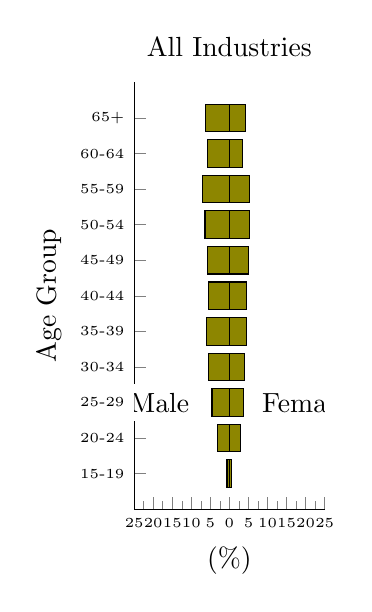
\begin{tikzpicture}
\begin{axis}[
    width=0.33\textwidth,
    height=7cm,
    xbar stacked,
    xmin=-25,
    xmax=25,
    xtick={-25, -20, -15, -10, -5, 0, 5, 10, 15, 20, 25},
    xticklabels={25, 20, 15, 10, 5, 0, 5, 10, 15, 20, 25},
    xlabel={(\%)},
    ylabel={Age Group},
    ytick={1,2,3,4,5,6,7,8,9,10,11},
    yticklabels={15-19, 20-24, 25-29, 30-34, 35-39, 40-44, 45-49, 50-54, 55-59, 60-64, 65+},
    title={All Industries},
    axis y line*=left,
    axis x line*=bottom,
    bar width=3.5mm,
    xticklabel style={font=\tiny},
    yticklabel style={font=\tiny},
    xlabel style={font=\normalsize},
    minor x tick num=1,
    grid style={line width=.1pt, draw=gray!20},
    major grid style={line width=.2pt,draw=gray!50},
]
\addplot[xbar, fill=olive] coordinates {(-6.2968,11) (-5.7348,10) (-7.0630,9) (-6.4160,8) (-5.8457,7) (-5.4109,6) (-6.0469,5) (-5.5079,4) (-4.5710,3) (-3.1366,2) (-0.6502,1)};
\addplot[xbar, fill=olive] coordinates {(4.1861,11) (3.5393,10) (5.1758,9) (5.2826,8) (4.9579,7) (4.4568,6) (4.5115,5) (4.0165,4) (3.6677,3) (2.9304,2) (0.5957,1)};
\node[anchor=east, fill=white] at (axis cs:-8,3) {Male};
\node[anchor=west, fill=white] at (axis cs:6,3) {Female};
\end{axis}
\end{tikzpicture}
\hfill
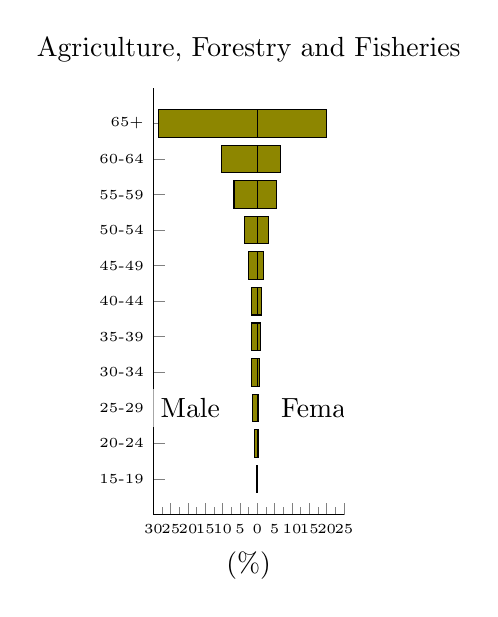
\begin{tikzpicture}
\begin{axis}[
    width=0.33\textwidth,
    height=7cm,
    xbar stacked,
    xmin=-30,
    xmax=25,
    xtick={-30, -25, -20, -15, -10, -5, 0, 5, 10, 15, 20, 25},
    xticklabels={30, 25, 20, 15, 10, 5, 0, 5, 10, 15, 20, 25},
    xlabel={(\%)},
    ytick={1,2,3,4,5,6,7,8,9,10,11},
    yticklabels={15-19, 20-24, 25-29, 30-34, 35-39, 40-44, 45-49, 50-54, 55-59, 60-64, 65+},
    yticklabel pos=right,
    title={Agriculture, Forestry and Fisheries},
    axis y line*=left,
    axis x line*=bottom,
    bar width=3.5mm,
    xticklabel style={font=\tiny},
    yticklabel style={font=\tiny},
    xlabel style={font=\normalsize},
    minor x tick num=1,
    grid style={line width=.1pt, draw=gray!20},
    major grid style={line width=.2pt,draw=gray!50},
]
\addplot[xbar, fill=olive] coordinates {(-28.5896,11) (-10.3951,10) (-6.7607,9) (-3.8248,8) (-2.5634,7) (-1.6352,6) (-1.6058,5) (-1.6520,4) (-1.2908,3) (-0.8218,2) (-0.1694,1)};
\addplot[xbar, fill=olive] coordinates {(20.0734,11) (6.5899,10) (5.5664,9) (3.2718,8) (1.7640,7) (1.1144,6) (0.8792,5) (0.6888,4) (0.4494,3) (0.2394,2) (0.0546,1)};
\node[anchor=east, fill=white] at (axis cs:-8,3) {Male};
\node[anchor=west, fill=white] at (axis cs:4,3) {Female};
\end{axis}
\end{tikzpicture}
\hfill
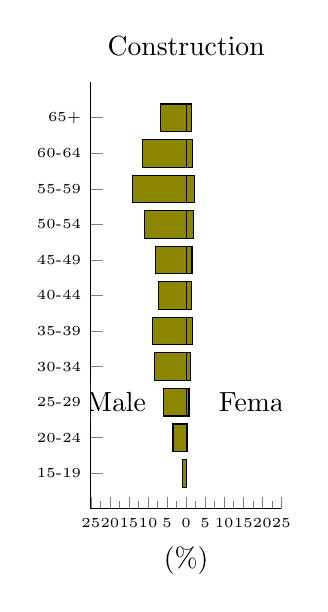
\begin{tikzpicture}
\begin{axis}[
    width=0.33\textwidth,
    height=7cm,
    xbar stacked,
    xmin=-25,
    xmax=25,
    xtick={-25, -20, -15, -10, -5, 0, 5, 10, 15, 20, 25},
    xticklabels={25, 20, 15, 10, 5, 0, 5, 10, 15, 20, 25},
    xlabel={(\%)},
    ytick={1,2,3,4,5,6,7,8,9,10,11},
    yticklabels={15-19, 20-24, 25-29, 30-34, 35-39, 40-44, 45-49, 50-54, 55-59, 60-64, 65+},
    yticklabel pos=right,
    title={Construction},
    axis y line*=left,
    axis x line*=bottom,
    bar width=3.5mm,
    xticklabel style={font=\tiny},
    yticklabel style={font=\tiny},
    xlabel style={font=\normalsize},
    minor x tick num=1,
    grid style={line width=.1pt, draw=gray!20},
    major grid style={line width=.2pt,draw=gray!50},
]
\addplot[xbar, fill=olive] coordinates {(-6.6875,11) (-11.4525,10) (-14.1118,9) (-10.9621,8) (-8.1361,7) (-7.1541,6) (-8.9182,5) (-8.3385,4) (-6.0411,3) (-3.4449,2) (-0.8749,1)};
\addplot[xbar, fill=olive] coordinates {(1.2939,11) (1.7058,10) (2.1069,9) (1.8165,8) (1.5332,7) (1.4439,6) (1.6165,5) (1.2035,4) (0.7380,3) (0.3726,2) (0.0476,1)};
\node[anchor=east, fill=white] at (axis cs:-8,3) {Male};
\node[anchor=west, fill=white] at (axis cs:6,3) {Female};
\end{axis}
\end{tikzpicture}
\end{adjustbox}

% 2行目のグラフ
\begin{adjustbox}{width=\textwidth}
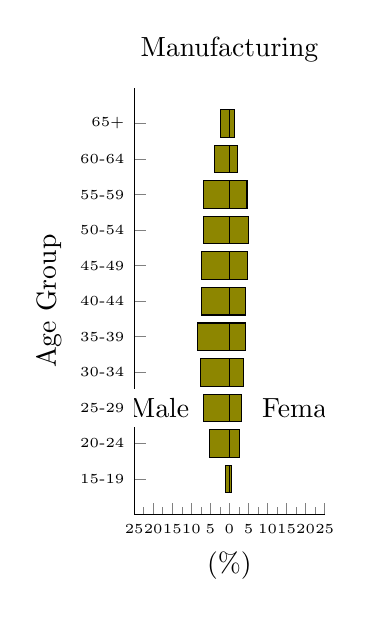
\begin{tikzpicture}
\begin{axis}[
    width=0.33\textwidth,
    height=7cm,
    xbar stacked,
    xmin=-25,
    xmax=25,
    xtick={-25, -20, -15, -10, -5, 0, 5, 10, 15, 20, 25},
    xticklabels={25, 20, 15, 10, 5, 0, 5, 10, 15, 20, 25},
    xlabel={(\%)},
    ylabel={Age Group},
    ytick={1,2,3,4,5,6,7,8,9,10,11},
    yticklabels={15-19, 20-24, 25-29, 30-34, 35-39, 40-44, 45-49, 50-54, 55-59, 60-64, 65+},
    title={Manufacturing},
    axis y line*=left,
    axis x line*=bottom,
    bar width=3.5mm,
    xticklabel style={font=\tiny},
    yticklabel style={font=\tiny},
    xlabel style={font=\normalsize},
    minor x tick num=1,
    grid style={line width=.1pt, draw=gray!20},
    major grid style={line width=.2pt,draw=gray!50},
]
\addplot[xbar, fill=olive] coordinates {(-2.4548,11) (-3.9043,10) (-6.7497,9) (-6.7481,8) (-7.4452,7) (-7.3451,6) (-8.3323,5) (-7.6527,4) (-6.7811,3) (-5.1740,2) (-0.9664,1)};
\addplot[xbar, fill=olive] coordinates {(1.2771,11) (2.1461,10) (4.6067,9) (4.9622,8) (4.8095,7) (4.2896,6) (4.3236,5) (3.6345,4) (3.1567,3) (2.7400,2) (0.5002,1)};
\node[anchor=east, fill=white] at (axis cs:-8,3) {Male};
\node[anchor=west, fill=white] at (axis cs:6,3) {Female};
\end{axis}
\end{tikzpicture}
\hfill
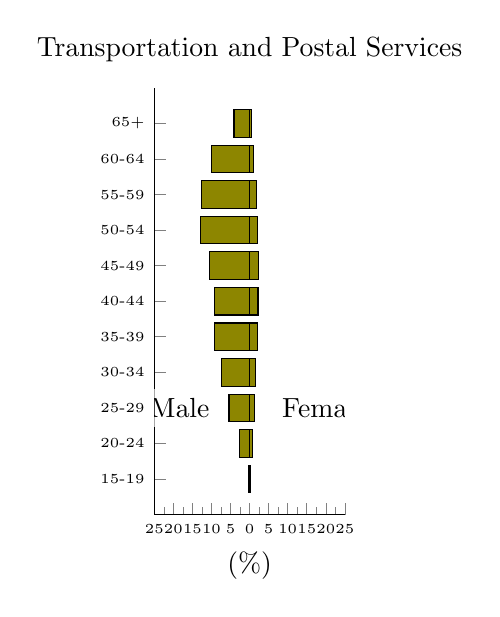
\begin{tikzpicture}
\begin{axis}[
    width=0.33\textwidth,
    height=7cm,
    xbar stacked,
    xmin=-25,
    xmax=25,
    xtick={-25, -20, -15, -10, -5, 0, 5, 10, 15, 20, 25},
    xticklabels={25, 20, 15, 10, 5, 0, 5, 10, 15, 20, 25},
    xlabel={(\%)},
    ytick={1,2,3,4,5,6,7,8,9,10,11},
    yticklabels={15-19, 20-24, 25-29, 30-34, 35-39, 40-44, 45-49, 50-54, 55-59, 60-64, 65+},
    yticklabel pos=right,
    title={Transportation and Postal Services},
    axis y line*=left,
    axis x line*=bottom,
    bar width=3.5mm,
    xticklabel style={font=\tiny},
    yticklabel style={font=\tiny},
    xlabel style={font=\normalsize},
    minor x tick num=1,
    grid style={line width=.1pt, draw=gray!20},
    major grid style={line width=.2pt,draw=gray!50},
]
\addplot[xbar, fill=olive] coordinates {(-4.0825,11) (-10.0013,10) (-12.6223,9) (-12.8891,8) (-10.6053,7) (-9.1725,6) (-9.1152,5) (-7.3627,4) (-5.4052,3) (-2.7445,2) (-0.3836,1)};
\addplot[xbar, fill=olive] coordinates {(0.5070,11) (1.0691,10) (1.8274,9) (2.1030,8) (2.3609,7) (2.2154,6) (2.0787,5) (1.4373,4) (1.1948,3) (0.7164,2) (0.1058,1)};
\node[anchor=east, fill=white] at (axis cs:-8,3) {Male};
\node[anchor=west, fill=white] at (axis cs:6,3) {Female};
\end{axis}
\end{tikzpicture}
\hfill
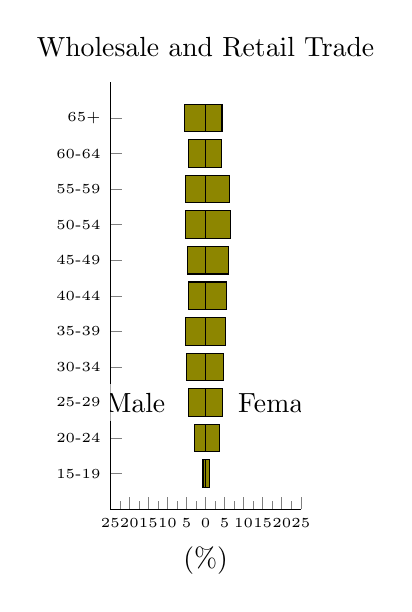
\begin{tikzpicture}
\begin{axis}[
    width=0.33\textwidth,
    height=7cm,
    xbar stacked,
    xmin=-25,
    xmax=25,
    xtick={-25, -20, -15, -10, -5, 0, 5, 10, 15, 20, 25},
    xticklabels={25, 20, 15, 10, 5, 0, 5, 10, 15, 20, 25},
    xlabel={(\%)},
    ytick={1,2,3,4,5,6,7,8,9,10,11},
    yticklabels={15-19, 20-24, 25-29, 30-34, 35-39, 40-44, 45-49, 50-54, 55-59, 60-64, 65+},
    yticklabel pos=right,
    title={Wholesale and Retail Trade},
    axis y line*=left,
    axis x line*=bottom,
    bar width=3.5mm,
    xticklabel style={font=\tiny},
    yticklabel style={font=\tiny},
    xlabel style={font=\normalsize},
    minor x tick num=1,
    grid style={line width=.1pt, draw=gray!20},
    major grid style={line width=.2pt,draw=gray!50},
]
\addplot[xbar, fill=olive] coordinates {(-5.6034,11) (-4.4603,10) (-5.3643,9) (-5.1647,8) (-4.7515,7) (-4.5047,6) (-5.3544,5) (-5.1161,4) (-4.4201,3) (-2.9335,2) (-0.6798,1)};
\addplot[xbar, fill=olive] coordinates {(4.3157,11) (4.1070,10) (6.2549,9) (6.4510,8) (6.0631,7) (5.4397,6) (5.2987,5) (4.7508,4) (4.3911,3) (3.5696,2) (1.0056,1)};
\node[anchor=east, fill=white] at (axis cs:-8,3) {Male};
\node[anchor=west, fill=white] at (axis cs:6,3) {Female};
\end{axis}
\end{tikzpicture}
\end{adjustbox}

% 3行目のグラフ
\begin{adjustbox}{width=\textwidth}
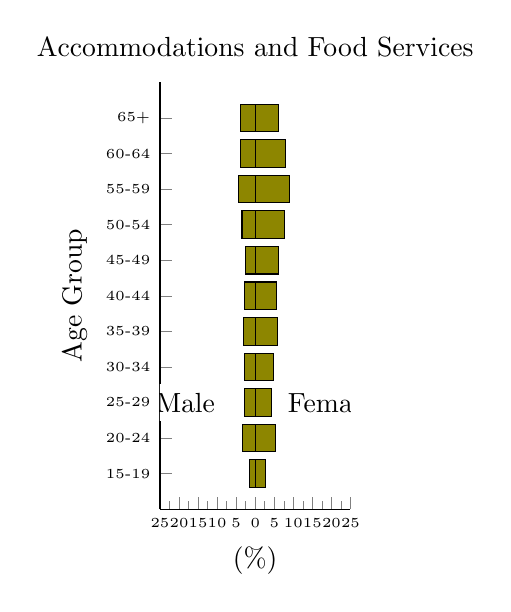
\begin{tikzpicture}
\begin{axis}[
    width=0.33\textwidth,
    height=7cm,
    xbar stacked,
    xmin=-25,
    xmax=25,
    xtick={-25, -20, -15, -10, -5, 0, 5, 10, 15, 20, 25},
    xticklabels={25, 20, 15, 10, 5, 0, 5, 10, 15, 20, 25},
 xlabel={(\%)},
    ylabel={Age Group},
    ytick={1,2,3,4,5,6,7,8,9,10,11},
    yticklabels={15-19, 20-24, 25-29, 30-34, 35-39, 40-44, 45-49, 50-54, 55-59, 60-64, 65+},
    title={Accommodations and Food Services},
    axis y line*=left,
    axis x line*=bottom,
    bar width=3.5mm,
    xticklabel style={font=\tiny},
    yticklabel style={font=\tiny},
    xlabel style={font=\normalsize},
    minor x tick num=1,
    grid style={line width=.1pt, draw=gray!20},
    major grid style={line width=.2pt,draw=gray!50},
]
\addplot[xbar, fill=olive] coordinates {(-3.8505,11) (-3.9093,10) (-4.2855,9) (-3.4547,8) (-2.6611,7) (-2.7884,6) (-3.0647,5) (-2.9217,4) (-2.9119,3) (-3.4410,2) (-1.4697,1)};
\addplot[xbar, fill=olive] coordinates {(6.1236,11) (7.9950,10) (9.0473,9) (7.6775,8) (6.0158,7) (5.6004,6) (5.7866,5) (4.7206,4) (4.3287,3) (5.2163,2) (2.7297,1)};
\node[anchor=east, fill=white] at (axis cs:-8,3) {Male};
\node[anchor=west, fill=white] at (axis cs:6,3) {Female};
\end{axis}
\end{tikzpicture}
\hfill
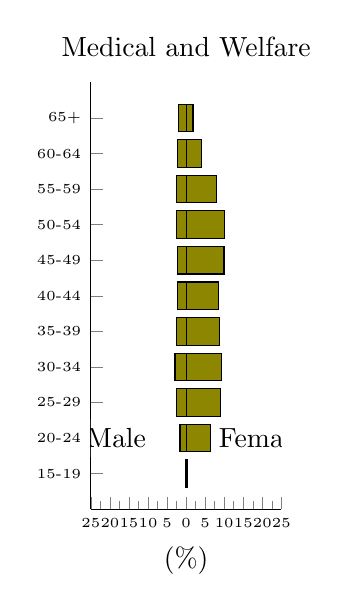
\begin{tikzpicture}
\begin{axis}[
    width=0.33\textwidth,
    height=7cm,
    xbar stacked,
    xmin=-25,
    xmax=25,
    xtick={-25, -20, -15, -10, -5, 0, 5, 10, 15, 20, 25},
    xticklabels={25, 20, 15, 10, 5, 0, 5, 10, 15, 20, 25},
    xlabel={(\%)},
    ytick={1,2,3,4,5,6,7,8,9,10,11},
    yticklabels={15-19, 20-24, 25-29, 30-34, 35-39, 40-44, 45-49, 50-54, 55-59, 60-64, 65+},
    yticklabel pos=right,
    title={Medical and Welfare},
    axis y line*=left,
    axis x line*=bottom,
    bar width=3.5mm,
    xticklabel style={font=\tiny},
    yticklabel style={font=\tiny},
    xlabel style={font=\normalsize},
    minor x tick num=1,
    grid style={line width=.1pt, draw=gray!20},
    major grid style={line width=.2pt,draw=gray!50},
]
\addplot[xbar, fill=olive] coordinates {(-2.0760,11) (-2.1576,10) (-2.4203,9) (-2.4234,8) (-2.3000,7) (-2.1796,6) (-2.5302,5) (-2.9330,4) (-2.5197,3) (-1.6072,2) (-0.1350,1)};
\addplot[xbar, fill=olive] coordinates {(1.8123,11) (4.0820,10) (8.0687,9) (10.0736,8) (9.9229,7) (8.4778,6) (8.8545,5) (9.3578,4) (9.1318,3) (6.4750,2) (0.4615,1)};
\node[anchor=east, fill=white] at (axis cs:-8,2) {Male};
\node[anchor=west, fill=white] at (axis cs:6,2) {Female};
\end{axis}
\end{tikzpicture}
\hfill
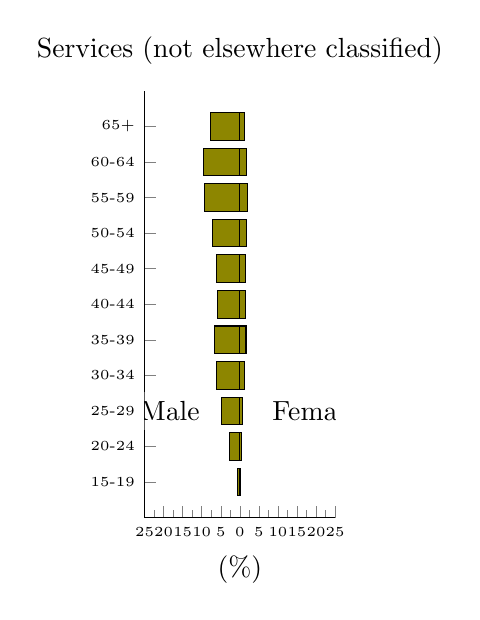
\begin{tikzpicture}
\begin{axis}[
    width=0.33\textwidth,
    height=7cm,
    xbar stacked,
    xmin=-25,
    xmax=25,
    xtick={-25, -20, -15, -10, -5, 0, 5, 10, 15, 20, 25},
    xticklabels={25, 20, 15, 10, 5, 0, 5, 10, 15, 20, 25},
    xlabel={(\%)},
    ytick={1,2,3,4,5,6,7,8,9,10,11},
    yticklabels={15-19, 20-24, 25-29, 30-34, 35-39, 40-44, 45-49, 50-54, 55-59, 60-64, 65+},
    yticklabel pos=right,
    title={Services (not elsewhere classified)},
    axis y line*=left,
    axis x line*=bottom,
    bar width=3.5mm,
    xticklabel style={font=\tiny},
    yticklabel style={font=\tiny},
    xlabel style={font=\normalsize},
    minor x tick num=1,
    grid style={line width=.1pt, draw=gray!20},
    major grid style={line width=.2pt,draw=gray!50},
]
\addplot[xbar, fill=olive] coordinates {(-7.5892,11) (-9.4724,10) (-9.3730,9) (-7.1919,8) (-6.1034,7) (-5.9352,6) (-6.6690,5) (-6.1825,4) (-4.8061,3) (-2.8135,2) (-0.5534,1)};
\addplot[xbar, fill=olive] coordinates {(1.2939,11) (1.7058,10) (2.1069,9) (1.8165,8) (1.5332,7) (1.4439,6) (1.6165,5) (1.2035,4) (0.7380,3) (0.3726,2) (0.0476,1)};
\node[anchor=east, fill=white] at (axis cs:-8,3) {Male};
\node[anchor=west, fill=white] at (axis cs:6,3) {Female};
\end{axis}
\end{tikzpicture}
\end{adjustbox}

\begin{flushleft}
\footnotesize
Source: Statistics Bureau, Ministry of Internal Affairs and Communications, Japan. "2010 Population Census."
\end{flushleft}


\caption{Proportion of Employed Persons Aged 15 and Over by Industry, Age (5-year groups), and Sex - Fukushima Pref. (2010)}
\label{fig:fukushima_Proportion_Employed}
\end{figure}

%%%%%%%%%%%%%%%%%%%%%%%%%%%%%%%%%%%%%%%%%%%%%

%福島県の職業(Occupation)別の男女別15歳以上就業者について、従業上の地位別(Employment type)の割合をみると、全職業(Total)では、男性の場合、「正規の職員・従業員」の割合は「事務従事者」が62.7%だが女性では40.1%である。一方、「パート・アルバイト・その他」の割合は、女性が36.8%に対して男性は9.8%である。自然災害が非正規労働者により大きな負の影響を及ぼすことが知られており、このような雇用形態のジェンダー格差は、そのまま自然災害影響のジェンダーギャップとして現れる。特筆すべきは、農林水産業では73.0%の男性が「Self-employed」と回答しているのに対し、女性の方は81.2%が「Family worker」と回答していることである。つまりFamily businessにおいては夫がオーナーであり、妻はその従業員であるという性別役割分担の存在が見てとれる。これは自然災害時に、夫よりも妻の労働の増減が危機に対する調整弁の役割を果たすことを意味する。


In Fukushima Prefecture, employment types among those aged 15 and over vary significantly by gender across occupations (Figure~\ref{fig:fukushima_Proportion_Occupation}). While 62.7\% of male clerical workers are regular employees, only 40.1\% of females are. Conversely, 36.8\% of women are part-time or temporary workers, compared to 9.8\% of men. This gender disparity in employment status can lead to disproportionate impacts during natural disasters. Notably, in agriculture, forestry, and fishery, 73.0\% of men are self-employed, while 81.2\% of women are family workers. This suggests a gendered division of labor in family businesses, where husbands are owners and wives are employees. Consequently, women's labor may serve as a buffer during crises, being more susceptible to fluctuations than men's.

%%%%%%%%%%%%%%%%%%%%%%%%%%%%%%%%%%%%%%%%%%%%%

\begin{figure}[!t]
\centering
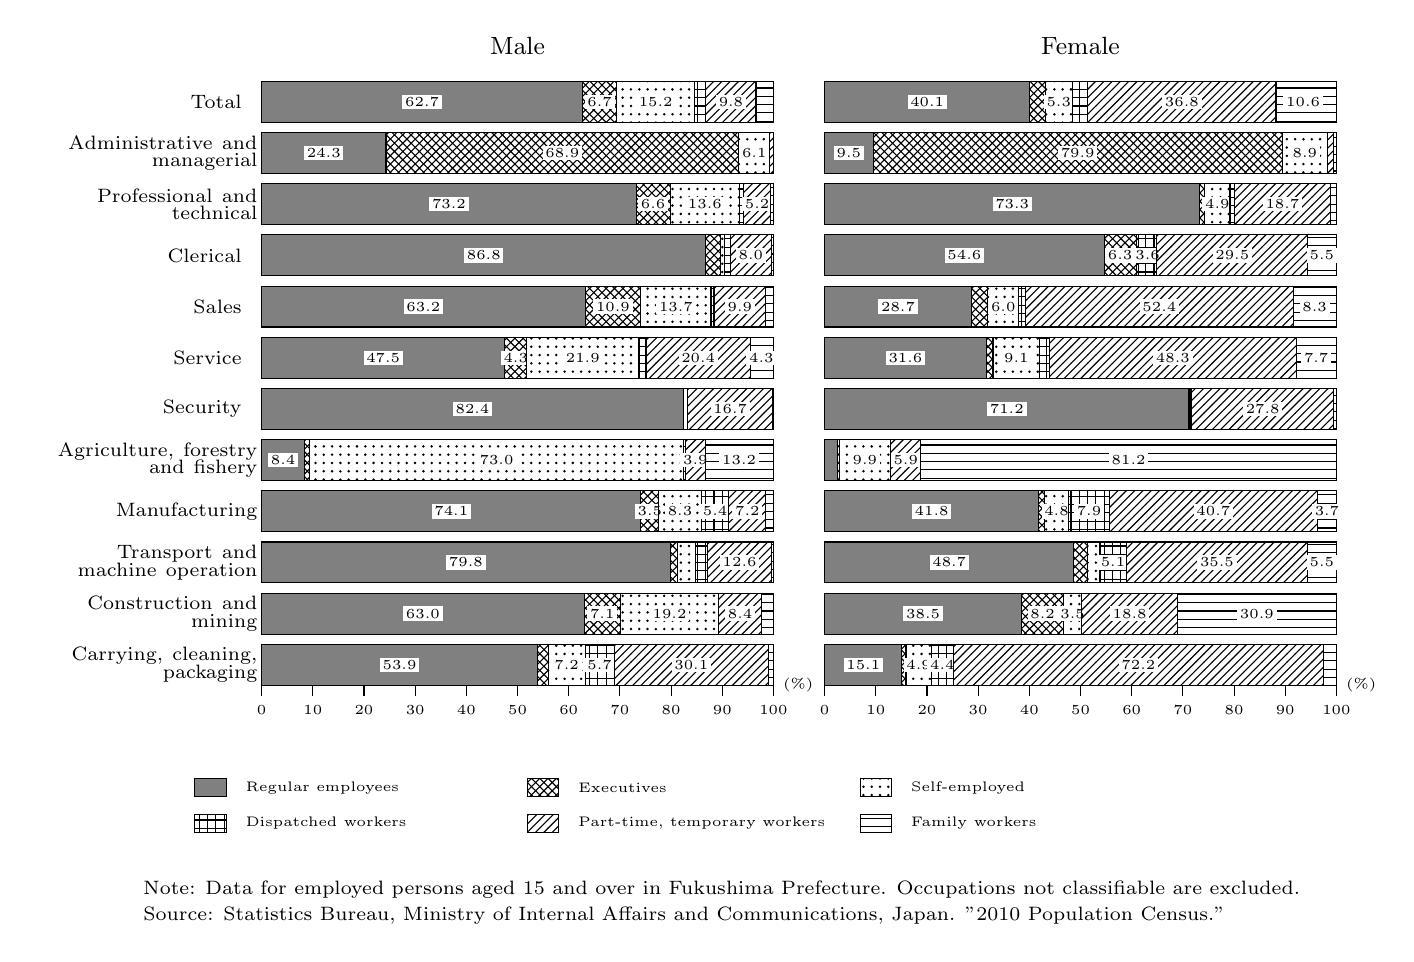
\begin{tikzpicture}[scale=0.65,xshift=-2cm]
\definecolor{color1}{RGB}{128,128,128}
\definecolor{color2}{RGB}{200,200,200}
\definecolor{color3}{RGB}{220,220,220}
\definecolor{color4}{RGB}{180,180,180}
\definecolor{color5}{RGB}{100,100,100}
\definecolor{color6}{RGB}{60,60,60}

% Function to draw a stacked bar
\newcommand{\stackedbar}[8]{
    \draw[fill=color1] (#1,#2) rectangle (#1+#3/10,#2+0.8);
    \pgfmathsetmacro{\result}{(#3 >= 3.5) ? 1 : 0}
    \ifnum\result>0
        \node[font=\tiny,fill=white,text=black,inner sep=1pt] at (#1+#3/20,#2+0.4) {#3};
    \fi
    \draw[fill=color2, pattern=crosshatch] (#1+#3/10,#2) rectangle (#1+#3/10+#4/10,#2+0.8);
    \pgfmathsetmacro{\result}{(#4 >= 3.5) ? 1 : 0}
    \ifnum\result>0
        \node[font=\tiny,fill=white,text=black,inner sep=1pt] at (#1+#3/10+#4/20,#2+0.4) {#4};
    \fi
    \draw[fill=color3, pattern=dots] (#1+#3/10+#4/10,#2) rectangle (#1+#3/10+#4/10+#5/10,#2+0.8);
    \pgfmathsetmacro{\result}{(#5 >= 3.5) ? 1 : 0}
    \ifnum\result>0
        \node[font=\tiny,fill=white,text=black,inner sep=1pt] at (#1+#3/10+#4/10+#5/20,#2+0.4) {#5};
    \fi
    \draw[fill=color4, pattern=grid] (#1+#3/10+#4/10+#5/10,#2) rectangle (#1+#3/10+#4/10+#5/10+#6/10,#2+0.8);
    \pgfmathsetmacro{\result}{(#6 >= 3.5) ? 1 : 0}
    \ifnum\result>0
        \node[font=\tiny,fill=white,text=black,inner sep=1pt] at (#1+#3/10+#4/10+#5/10+#6/20,#2+0.4) {#6};
    \fi
    \draw[fill=color5, pattern=north east lines] (#1+#3/10+#4/10+#5/10+#6/10,#2) rectangle (#1+#3/10+#4/10+#5/10+#6/10+#7/10,#2+0.8);
    \pgfmathsetmacro{\result}{(#7 >= 3.5) ? 1 : 0}
    \ifnum\result>0
        \node[font=\tiny,fill=white,text=black,inner sep=1pt] at (#1+#3/10+#4/10+#5/10+#6/10+#7/20,#2+0.4) {#7};
    \fi
    \draw[fill=color6, pattern=horizontal lines] (#1+#3/10+#4/10+#5/10+#6/10+#7/10,#2) rectangle (#1+10,#2+0.8);
    \pgfmathsetmacro{\result}{(#8 >= 3.5) ? 1 : 0}
    \ifnum\result>0
        \node[font=\tiny,fill=white,text=black,inner sep=1pt] at (#1+#3/10+#4/10+#5/10+#6/10+#7/10+#8/20,#2+0.4) {#8};
    \fi
}

% Male bars
\begin{scope}[xshift=-5.5cm]
\stackedbar{0}{11}{62.7}{6.7}{15.2}{2.2}{9.8}{2.3}
\node[anchor=east, text width=2.6cm, align=right] at (-0.2,11.4) {\scriptsize Total};
\stackedbar{0}{10}{24.3}{68.9}{6.1}{0}{0.7}{0}
\node[anchor=east, text width=2.6cm, align=right] at (-0.2,10.4) {\scriptsize\parbox[t]{2.8cm}{\setstretch{0.8}\raggedleft Administrative and managerial}};
\stackedbar{0}{9}{73.2}{6.6}{13.6}{0.8}{5.2}{0.6}
\node[anchor=east, text width=2.6cm, align=right] at (-0.2,9.4) {\scriptsize\parbox[t]{2.8cm}{\setstretch{0.8}\raggedleft Professional and technical}};
\stackedbar{0}{8}{86.8}{2.9}{0.7}{1.2}{8.0}{0.3}
\node[anchor=east, text width=2.6cm, align=right] at (-0.2,8.4) {\scriptsize Clerical};
\stackedbar{0}{7}{63.2}{10.9}{13.7}{0.7}{9.9}{1.6}
\node[anchor=east, text width=2.6cm, align=right] at (-0.2,7.4) {\scriptsize Sales};
\stackedbar{0}{6}{47.5}{4.3}{21.9}{1.4}{20.4}{4.3}
\node[anchor=east, text width=2.6cm, align=right] at (-0.2,6.4) {\scriptsize Service};
\stackedbar{0}{5}{82.4}{0.1}{0.7}{0}{16.7}{0}
\node[anchor=east, text width=2.6cm, align=right] at (-0.2,5.4) {\scriptsize Security};
\stackedbar{0}{4}{8.4}{1.0}{73.0}{0.4}{3.9}{13.2}
\node[anchor=east, text width=2.6cm, align=right] at (-0.2,4.4) {\scriptsize\parbox[t]{2.8cm}{\setstretch{0.8}\raggedleft Agriculture, forestry and fishery}};
\stackedbar{0}{3}{74.1}{3.5}{8.3}{5.4}{7.2}{1.4}
\node[anchor=east, text width=2.6cm, align=right] at (-0.2,3.4) {\scriptsize\parbox[t]{2.8cm}{\setstretch{0.8}\raggedleft Manufacturing}};
\stackedbar{0}{2}{79.8}{1.5}{3.4}{2.4}{12.6}{0.2}
\node[anchor=east, text width=2.6cm, align=right] at (-0.2,2.4) {\scriptsize\parbox[t]{2.8cm}{\setstretch{0.8}\raggedleft Transport and machine operation}};
\stackedbar{0}{1}{63.0}{7.1}{19.2}{0}{8.4}{2.2}
\node[anchor=east, text width=2.6cm, align=right] at (-0.2,1.4) {\scriptsize\parbox[t]{2.8cm}{\setstretch{0.8}\raggedleft Construction and mining}};
\stackedbar{0}{0}{53.9}{2.1}{7.2}{5.7}{30.1}{1.0}
\node[anchor=east, text width=2.6cm, align=right] at (-0.2,0.4) {\scriptsize\parbox[t]{2.8cm}{\setstretch{0.8}\raggedleft Carrying, cleaning, packaging}};

% X-axis for Male
\draw (0,0) -- (10,0);
\foreach \x in {0,1,...,10}
    \draw (\x,0) -- (\x,-0.2) node[anchor=north] {\tiny \ifnum\x=0 0\else\x0\fi};
\node[anchor=west] at (10,0) {\tiny (\%)};

% Label for Male
\node[anchor=center] at (5,12.5) {\small Male};
\end{scope}

% Female bars
\begin{scope}[xshift=5.5cm]
\stackedbar{0}{11}{40.1}{3.0}{5.3}{3.0}{36.8}{10.6}
\stackedbar{0}{10}{9.5}{79.9}{8.9}{0}{1.1}{0.6}
\stackedbar{0}{9}{73.3}{1.0}{4.9}{0.9}{18.7}{1.2}
\stackedbar{0}{8}{54.6}{6.3}{0.4}{3.6}{29.5}{5.5}
\stackedbar{0}{7}{28.7}{3.2}{6.0}{1.3}{52.4}{8.3}
\stackedbar{0}{6}{31.6}{1.3}{9.1}{1.9}{48.3}{7.7}
\stackedbar{0}{5}{71.2}{0.2}{0.3}{0}{27.8}{0}
\stackedbar{0}{4}{2.5}{0.4}{9.9}{0.1}{5.9}{81.2}
\stackedbar{0}{3}{41.8}{1.1}{4.8}{7.9}{40.7}{3.7}
\stackedbar{0}{2}{48.7}{2.7}{2.4}{5.1}{35.5}{5.5}
\stackedbar{0}{1}{38.5}{8.2}{3.5}{0}{18.8}{30.9}
\stackedbar{0}{0}{15.1}{0.8}{4.9}{4.4}{72.2}{2.6}

% X-axis for Female
\draw (0,0) -- (10,0);
\foreach \x in {0,1,...,10}
    \draw (\x,0) -- (\x,-0.2) node[anchor=north] {\tiny \ifnum\x=0 0\else\x0\fi};
\node[anchor=west] at (10,0) {\tiny (\%)};

% Label for Female
\node[anchor=center] at (5,12.5) {\small Female};
\end{scope}

% Legend (2 rows, 3 columns)
\node[anchor=center, fill=color1, minimum width=0.4cm, minimum height=0.2cm, draw] at (-6.5,-2) {};
\node[anchor=west] at (-6,-2) {\tiny Regular employees};
\node[anchor=center, fill=color2, pattern=crosshatch, minimum width=0.4cm, minimum height=0.2cm, draw] at (0,-2) {};
\node[anchor=west] at (0.5,-2) {\tiny Executives};
\node[anchor=center, fill=color3, pattern=dots, minimum width=0.4cm, minimum height=0.2cm, draw] at (6.5,-2) {};
\node[anchor=west] at (7,-2) {\tiny Self-employed};
\node[anchor=center, fill=color4, pattern=grid, minimum width=0.4cm, minimum height=0.2cm, draw] at (-6.5,-2.7) {};
\node[anchor=west] at (-6,-2.7) {\tiny Dispatched workers};
\node[anchor=center, fill=color5, pattern=north east lines, minimum width=0.4cm, minimum height=0.2cm, draw] at (0,-2.7) {};
\node[anchor=west] at (0.5,-2.7) {\tiny Part-time, temporary workers};
\node[anchor=center, fill=color6, pattern=horizontal lines, minimum width=0.4cm, minimum height=0.2cm, draw] at (6.5,-2.7) {};
\node[anchor=west] at (7,-2.7) {\tiny Family workers};

% Note and Source
\node[anchor=west] at (-8,-4) {\scriptsize Note: Data for employed persons aged 15 and over in Fukushima Prefecture. Occupations not classifiable are excluded.};
\node[anchor=west] at (-8,-4.5) {\scriptsize Source: Statistics Bureau, Ministry of Internal Affairs and Communications, Japan. "2010 Population Census."};

\end{tikzpicture}
\caption{Proportion of Employed Persons Aged 15 and Over by Occupation, Employment types, and Gender - Fukushima Pref. (2010)}
\label{fig:fukushima_Proportion_Occupation}
\end{figure}

%%%%%%%%%%%%%%%%%%%%%%%%%%%%%%%%%%%%%%%%%%%%%


\subsection{The Impact of Evacuation on Labour Force}
\label{sec4.1}
The nuclear accident triggered significant demographic shifts in Fukushima Prefecture. Immediately following the disaster, evacuation orders covered approximately 12\% of the prefecture's area, encompassing 12 municipalities surrounding the Fukushima nuclear power plant. This led to long-term and widespread displacement of residents both within and outside the prefecture\footnote{As of 2024, the area designated as "difficult-to-return zones" has been reduced to 2.2\%, of the prefecture’s area.}.


According to the Reconstruction Agency, the number of evacuees from Fukushima Prefecture was reported as 59,464 (2.9\% of Fukushima's total population) as of December 2011, nine months after the earthquake. Additionally, the number of evacuees within Fukushima Prefecture was 95,200. Therefore, a total of 154,664 people (7.6\% of Fukushima's total population) became evacuees, and this number still stood at 110,880 five years after the disaster.

%Consequently, the monthly effective job openings-to-applicants ratio rose to 0.70 in November 2011, surpassing the national average of 0.69 for the first time in 10 years and 6 months.

As shown in Figure~\ref{fig:number_of_net_migration}, the official net migration plummeted to -31,381 in 2011 and -13,843 in 2012\footnote{The net migration data is sourced from the 'Basic Resident Registration Population Migration Report' by the Statistics Bureau, Ministry of Internal Affairs and Communications. It is important to note that these figures only account for individuals who officially reported their relocation to administrative agencies. There were likely many evacuees who did not formally register their moves.}. This exodus was most pronounced among children under 15 and adults aged 25-44, likely representing family units. Notably, female outmigration surpassed that of male in the 25-44 age group, corroborated by substantial decreases in kindergarten and elementary school enrollments. This pattern suggests a disproportionate evacuation of children and mothers due to nuclear safety concerns. However, by 2014-2015, a partial reversal emerged, characterized by net positive male migration, indicating a gender-imbalanced return trend. The proportion of female net out-migration to total net out-migration in 2014 and 2015 surged to 140.2\% and 122.4\% respectively, indicating a larger positive net migration for males than females. This complex migration pattern underscores the profound and lasting demographic impact of the disaster on Fukushima, with initial family-centric outmigration followed by a male-led return phase.

\begin{figure}[h!]
    \centering
    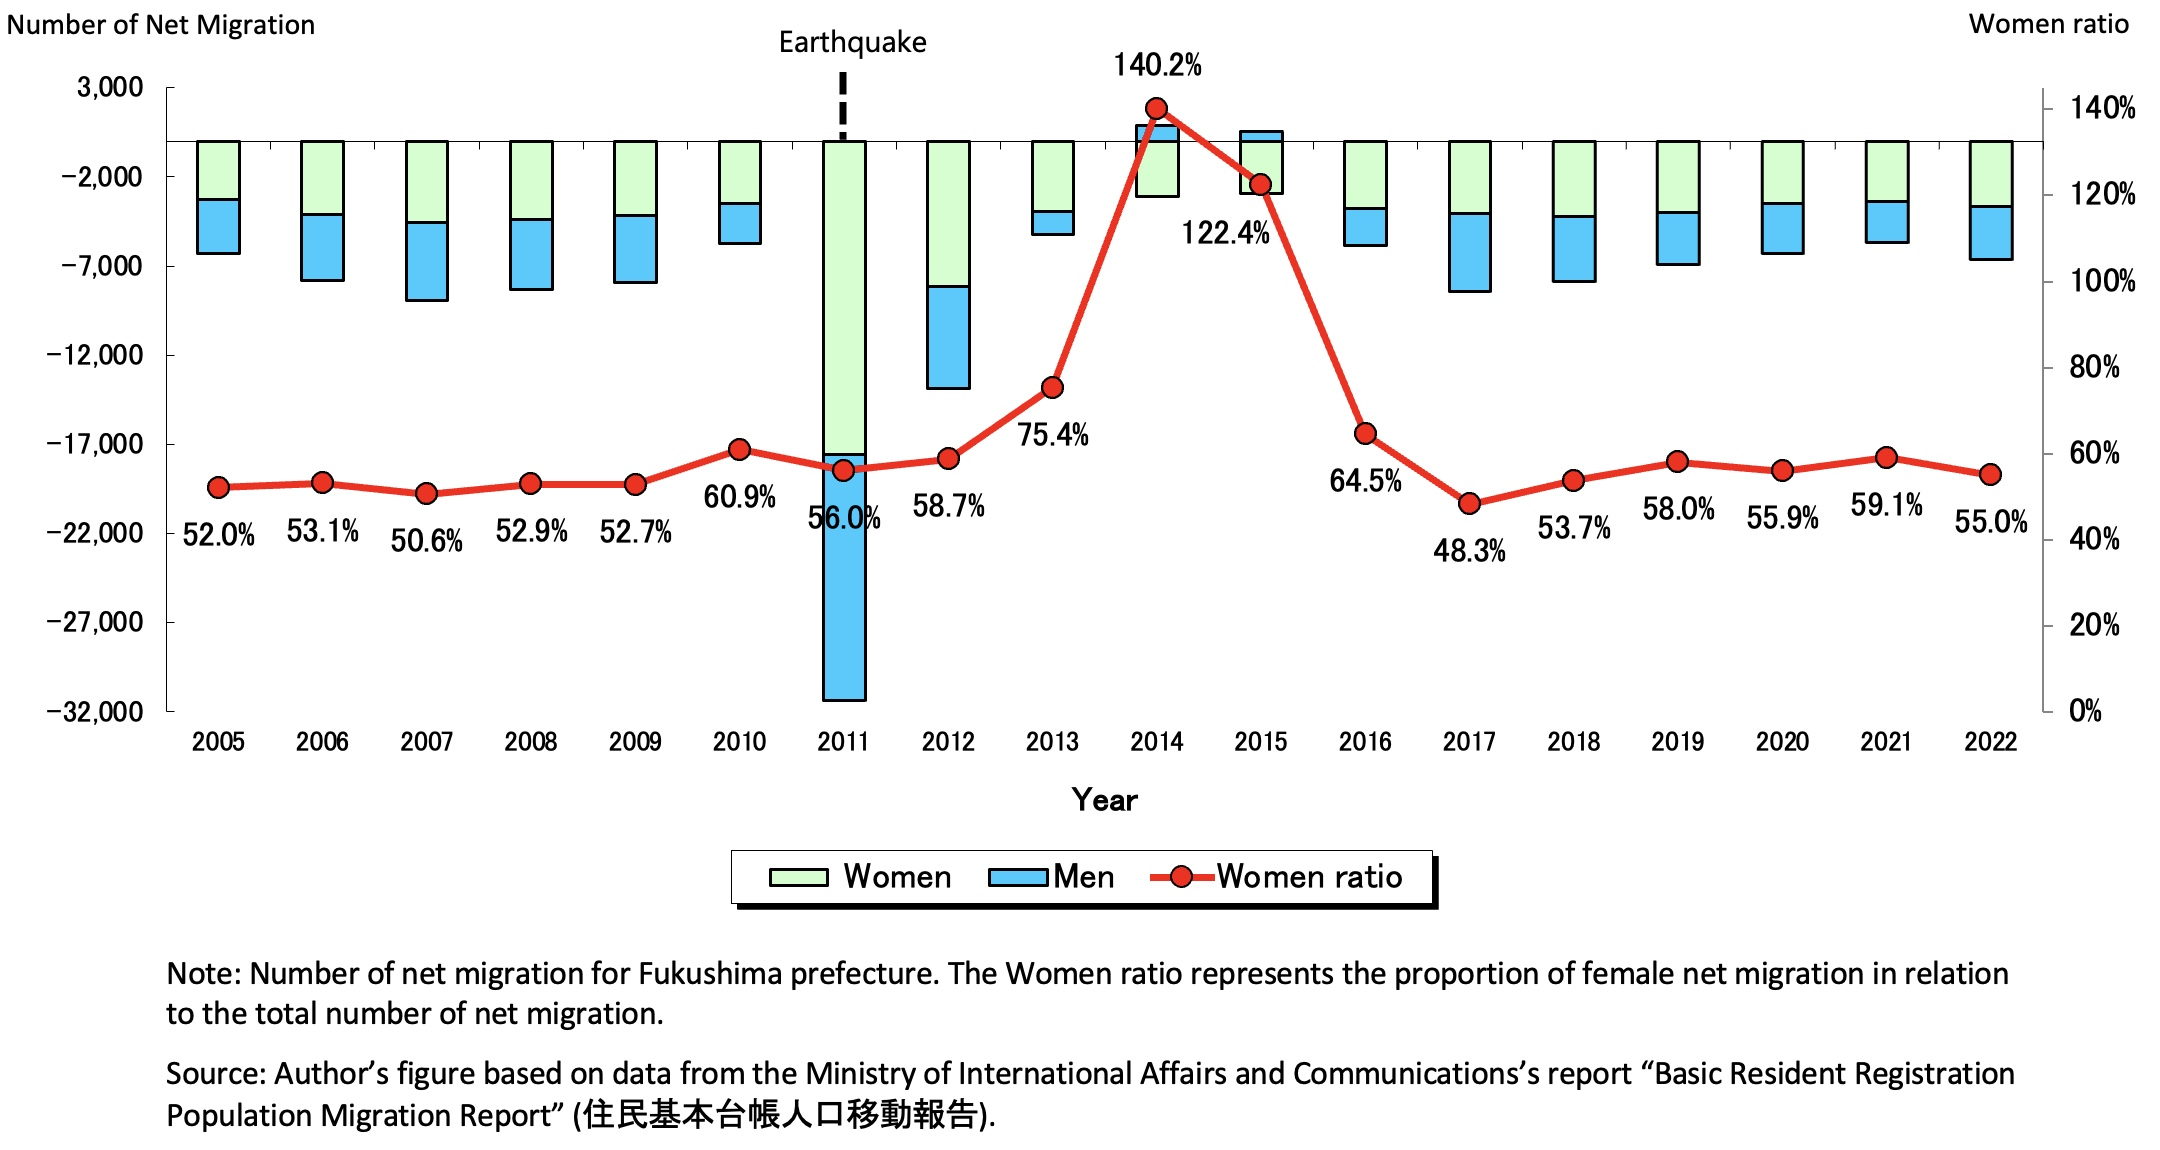
\includegraphics[width=0.9\textwidth]{Number of net migration.jpeg}  % 幅を本文の80%に設定
    \caption{The Number of Net Migration and The Proportion of Female Net Out-migration to Total Net Out-migration in Fukushima Pref.}
    \label{fig:number_of_net_migration}
\end{figure}

\clearpage

\subsection{Labour Force Participation Rate in Fukushima pref}
\label{sec4.1}


Did women's labor force participation in Fukushima Prefecture increase more than the national average after the disaster?
The large-scale outmigration of working-age population (25-44 years old), especially women, potentially affected the labor force participation rate (the ratio of the labor force to the working-age population aged 15-64). Figure~\ref{fig:fukushima_labour_force_participation_rate} compares Fukushima's labor force participation rates to the national average before and after the 2011 earthquake. The data shows no evidence of a greater increase in Fukushima's female rates compared to the national average between pre-disaster (2010) and post-disaster periods (2015 and 2020). In fact, the national average increased more during this period.


%%%%%%%%%%%%%%%%%%%%%%%%%%%%%%%%%%%%%%%%%%%%

\begin{figure}[h!]

\begin{subfigure}{\textwidth}
\caption{Fukushima Pref.}
\begin{minipage}{0.48\textwidth}
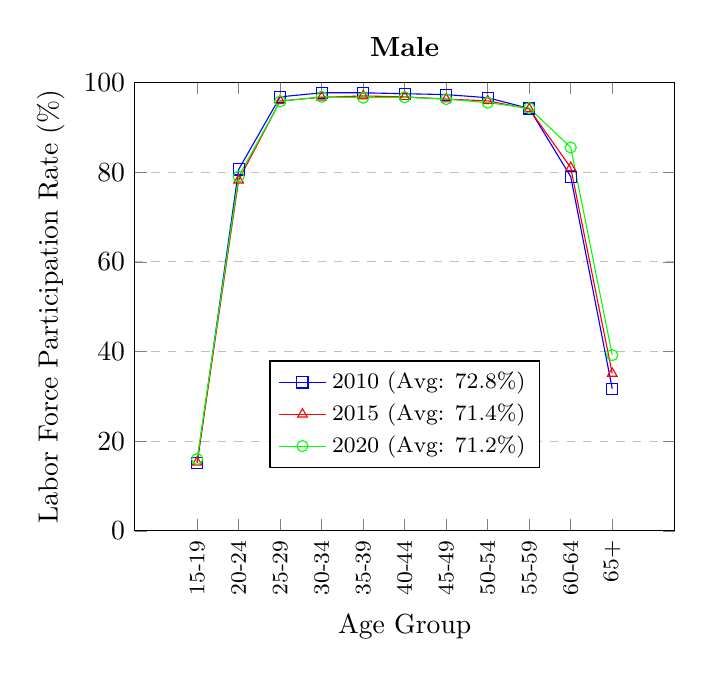
\begin{tikzpicture}
\begin{axis}[
    title={\textbf{Male}},
    xlabel={Age Group},
    ylabel={Labor Force Participation Rate (\%)},
    xmin=0, xmax=12,
    ymin=0, ymax=100,
    xtick={1,2,3,4,5,6,7,8,9,10,11},
    xticklabels={15-19,20-24,25-29,30-34,35-39,40-44,45-49,50-54,55-59,60-64,65+},
    x tick label style={rotate=90,anchor=east,font=\footnotesize},
    legend style={at={(0.5,0.38)},anchor=north,font=\footnotesize,
                  cells={anchor=west},
                  legend columns=1,
                  draw=black,fill=white,align=left},
    ymajorgrids=true,
    grid style=dashed,
    enlarge x limits={abs=0.5},
]

\addplot[color=blue,mark=square,] coordinates {
    (1,15.1)(2,80.6)(3,96.8)(4,97.7)(5,97.7)(6,97.5)(7,97.3)(8,96.6)(9,94.2)(10,79.0)(11,31.7)
};

\addplot[color=red,mark=triangle,] coordinates {
    (1,15.3)(2,78.2)(3,95.9)(4,96.7)(5,97.0)(6,96.8)(7,96.3)(8,95.9)(9,94.1)(10,81.0)(11,35.1)
};

\addplot[color=green,mark=o,] coordinates {
    (1,16.0)(2,79.0)(3,95.8)(4,96.8)(5,96.6)(6,96.7)(7,96.3)(8,95.5)(9,94.3)(10,85.5)(11,39.2)
};

\legend{
    2010 (Avg: 72.8\%),
    2015 (Avg: 71.4\%),
    2020 (Avg: 71.2\%)
}
\end{axis}
\end{tikzpicture}
\end{minipage}
\hfill
\begin{minipage}{0.48\textwidth}
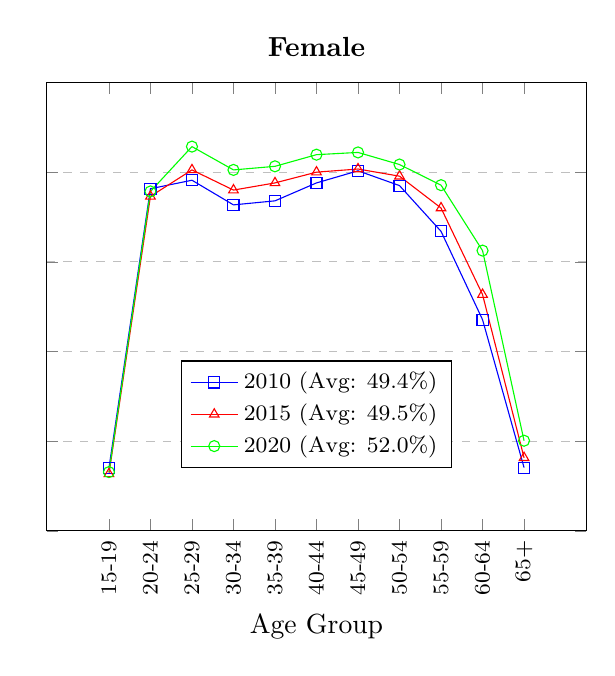
\begin{tikzpicture}
\begin{axis}[
    title={\textbf{Female}},
    xlabel={Age Group},
    ylabel={},
    xmin=0, xmax=12,
    ymin=0, ymax=100,
    xtick={1,2,3,4,5,6,7,8,9,10,11},
    xticklabels={15-19,20-24,25-29,30-34,35-39,40-44,45-49,50-54,55-59,60-64,65+},
    x tick label style={rotate=90,anchor=east,font=\footnotesize},
    legend style={at={(0.5,0.38)},anchor=north,font=\footnotesize,
                  cells={anchor=west},
                  legend columns=1,
                  draw=black,fill=white,align=left},
    ymajorgrids=true,
    grid style=dashed,
    yticklabels={,,},
    enlarge x limits={abs=0.5},
]

\addplot[color=blue,mark=square,] coordinates {
    (1,14.0)(2,76.3)(3,78.2)(4,72.7)(5,73.6)(6,77.6)(7,80.3)(8,77.0)(9,66.8)(10,47.1)(11,14.1)
};

\addplot[color=red,mark=triangle,] coordinates {
    (1,12.7)(2,74.6)(3,80.5)(4,76.0)(5,77.6)(6,80.0)(7,80.7)(8,79.1)(9,72.0)(10,52.7)(11,16.3)
};

\addplot[color=green,mark=o,] coordinates {
    (1,13.1)(2,75.7)(3,85.7)(4,80.5)(5,81.3)(6,83.9)(7,84.4)(8,81.7)(9,77.1)(10,62.5)(11,20.1)
};

\legend{
    2010 (Avg: 49.4\%),
    2015 (Avg: 49.5\%),
    2020 (Avg: 52.0\%)
}
\end{axis}
\end{tikzpicture}
\end{minipage}
\end{subfigure}

\vspace{0.5cm}

\begin{subfigure}{\textwidth}
\caption{Nationwide}
\begin{minipage}{0.48\textwidth}
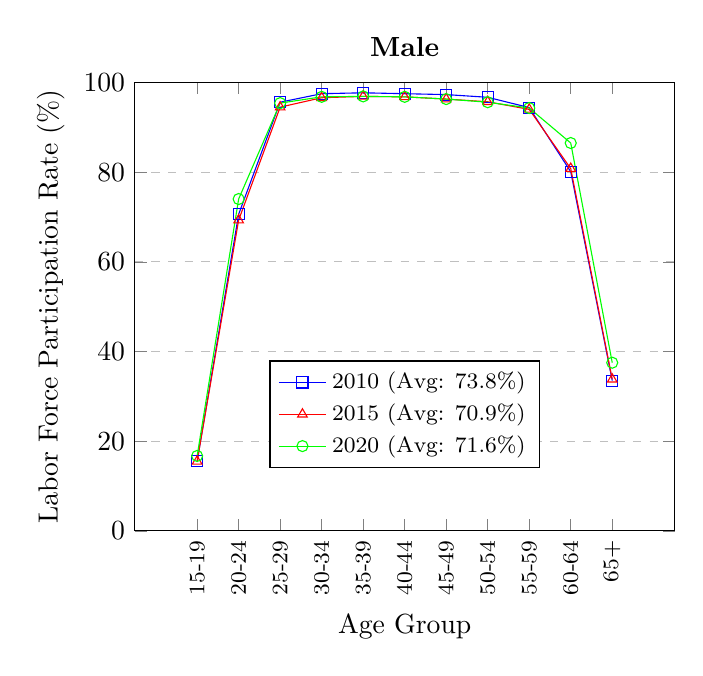
\begin{tikzpicture}
\begin{axis}[
    title={\textbf{Male}},
    xlabel={Age Group},
    ylabel={Labor Force Participation Rate (\%)},
    xmin=0, xmax=12,
    ymin=0, ymax=100,
    xtick={1,2,3,4,5,6,7,8,9,10,11},
    xticklabels={15-19,20-24,25-29,30-34,35-39,40-44,45-49,50-54,55-59,60-64,65+},
    x tick label style={rotate=90,anchor=east,font=\footnotesize},
    legend style={at={(0.5,0.38)},anchor=north,font=\footnotesize,
                  cells={anchor=west},
                  legend columns=1,
                  draw=black,fill=white,align=left},
    ymajorgrids=true,
    grid style=dashed,
    enlarge x limits={abs=0.5},
]

\addplot[color=blue,mark=square,] coordinates {
    (1,15.5)(2,70.6)(3,95.6)(4,97.5)(5,97.7)(6,97.5)(7,97.3)(8,96.7)(9,94.4)(10,80.1)(11,33.5)
};

\addplot[color=red,mark=triangle,] coordinates {
    (1,15.5)(2,69.3)(3,94.5)(4,96.6)(5,96.9)(6,96.8)(7,96.3)(8,95.7)(9,94.0)(10,80.8)(11,33.8)
};

\addplot[color=green,mark=o,] coordinates {
    (1,16.7)(2,74.0)(3,95.4)(4,96.8)(5,96.9)(6,96.8)(7,96.3)(8,95.6)(9,94.3)(10,86.5)(11,37.5)
};

\legend{
    2010 (Avg: 73.8\%),
    2015 (Avg: 70.9\%),
    2020 (Avg: 71.6\%)
}
\end{axis}
\end{tikzpicture}
\end{minipage}
\hfill
\begin{minipage}{0.48\textwidth}
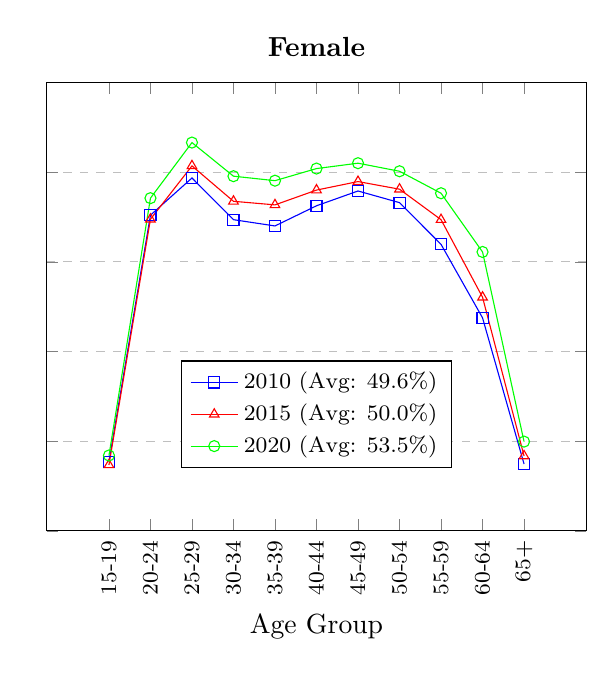
\begin{tikzpicture}
\begin{axis}[
    title={\textbf{Female}},
    xlabel={Age Group},
    ylabel={},
    xmin=0, xmax=12,
    ymin=0, ymax=100,
    xtick={1,2,3,4,5,6,7,8,9,10,11},
    xticklabels={15-19,20-24,25-29,30-34,35-39,40-44,45-49,50-54,55-59,60-64,65+},
    x tick label style={rotate=90,anchor=east,font=\footnotesize},
    legend style={at={(0.5,0.38)},anchor=north,font=\footnotesize,
                  cells={anchor=west},
                  legend columns=1,
                  draw=black,fill=white,align=left},
    ymajorgrids=true,
    grid style=dashed,
    yticklabels={,,},
    enlarge x limits={abs=0.5},
]

\addplot[color=blue,mark=square,] coordinates {
    (1,15.4)(2,70.4)(3,78.7)(4,69.4)(5,68.0)(6,72.5)(7,75.8)(8,73.2)(9,63.9)(10,47.5)(11,14.9)
};

\addplot[color=red,mark=triangle,] coordinates {
    (1,14.7)(2,69.5)(3,81.4)(4,73.5)(5,72.7)(6,76.0)(7,77.9)(8,76.2)(9,69.4)(10,52.1)(11,16.7)
};

\addplot[color=green,mark=o,] coordinates {
    (1,16.8)(2,74.2)(3,86.6)(4,79.1)(5,78.1)(6,80.8)(7,82.0)(8,80.2)(9,75.3)(10,62.2)(11,19.9)
};

\legend{
    2010 (Avg: 49.6\%),
    2015 (Avg: 50.0\%),
    2020 (Avg: 53.5\%)
}
\end{axis}
\end{tikzpicture}
\end{minipage}
\end{subfigure}

\vspace{0.5cm}

\begin{minipage}{\textwidth}
\footnotesize
\textbf{Note:} Labor force participation rates from the 2010, 2015, and 2020 Population Censuses. The ratio of the labor force to the population aged 15 and over (excluding those with "unknown" labor force status).

\end{minipage}


\caption{Labour Force Participation Rate by Age (Five-Year Groups) and Sex - Fukushima Pref/Japan}


\label{fig:fukushima_labour_force_participation_rate}

\end{figure}

%%%%%%%%%%%%%%%%%%%%%%%%%%%%%%%%%%%%%%%%%%%%%



\clearpage
\subsection{Job Openings/Applicants Analysis}
\label{sec4.1}

The disaster resulted in an exceptionally grave employment situation. Initially, there was a sharp increase in job seekers and unemployment insurance recipients. However, the employment situation gradually improved, primarily due to an upsurge in job openings related to post-disaster reconstruction, particularly in the construction sector. 


Figure~\ref{fig:new_job_openings} illustrates the number of new job openings/applicants and trends in the Effective Job Openings-to-Applicants Ratio in Fukushima Prefecture and Nationwide, recorded at Hello Work, Japan’s public employment security office, which maintains a comprehensive database of current job vacancies accessible to all citizens\footnote{It should be noted that Hello Work job listings represent only a partial view of the overall labor market. According to the Ministry of Health, Labour and Welfare's "Survey on Employment Trends," in 2013, out of 7.49 million new hires nationwide, 35.8\% were through media/advertising, 21.8\% through personal connections, and 20.2\% through Hello Work. Recently, high-income white-collar positions increasingly use online platforms or direct hiring rather than Hello Work. Hello Work listings may be skewed towards certain sectors, such as healthcare and social welfare. Additionally, Hello Work is more commonly used for recruitment in small and medium-sized enterprises.}. 

%「Hello Workの求人・求職情報は、労働市場全体の一部を表しているに過ぎないことに留意が必要。厚生労働省「雇用動向調査」によれば、日本全国の平成25年の入職者数は749万人(一般労働者:426万、パートタイム労働者:323万人)で、その入職経路をみると、求人メディア・広告によるものが268万人(35.8%)と最も多く、次いで縁故の163万人(21.8%)、ハローワークの151万人(20.2%)となっている。また、最近では高年収のホワイトカラー職種などでは、ハローワークではなく、ビジネスSNSや人材データベースなどのネット求人や企業が直接採用を行うケースが増えてきている。ハローワークでは医療・福祉分野の求人が多いなど、職種による偏りがあることにも留意が必要。また、ハローワークは中小企業入職者で、media/advertisingは大企業入職者で多い。」

%注)『一般職業紹介状況(職業安定業務統計)』は「全国の公共職業安定所(ハローワーク)における職業紹介業務の実績を集計した業務統計」である。厚生労働省『平成22年雇用動向調査』によれば、入職者に占める公共職業安定所が入職経路である者は21.5%(ハローワークインターネットサービスを含むと26.2%)であること,また,管理的職業など,公共職業安定所を経路としない職業など,分析対象と成る職業に偏りがあることを留意する必要がある。


After the 2011 earthquake, Fukushima's job openings-to-applicants ratio surpassed the national average until 2016, driven by a reconstruction boom. This led to a sharp increase in job openings, especially in restoration projects. Post-2016, as reconstruction demand peaked, the ratio fell below the national average. Job openings remained high but declining, while applications steadily decreased, indicating increased employment absorption due to continuous high job openings situation.


\begin{figure}[h!]
    \centering
    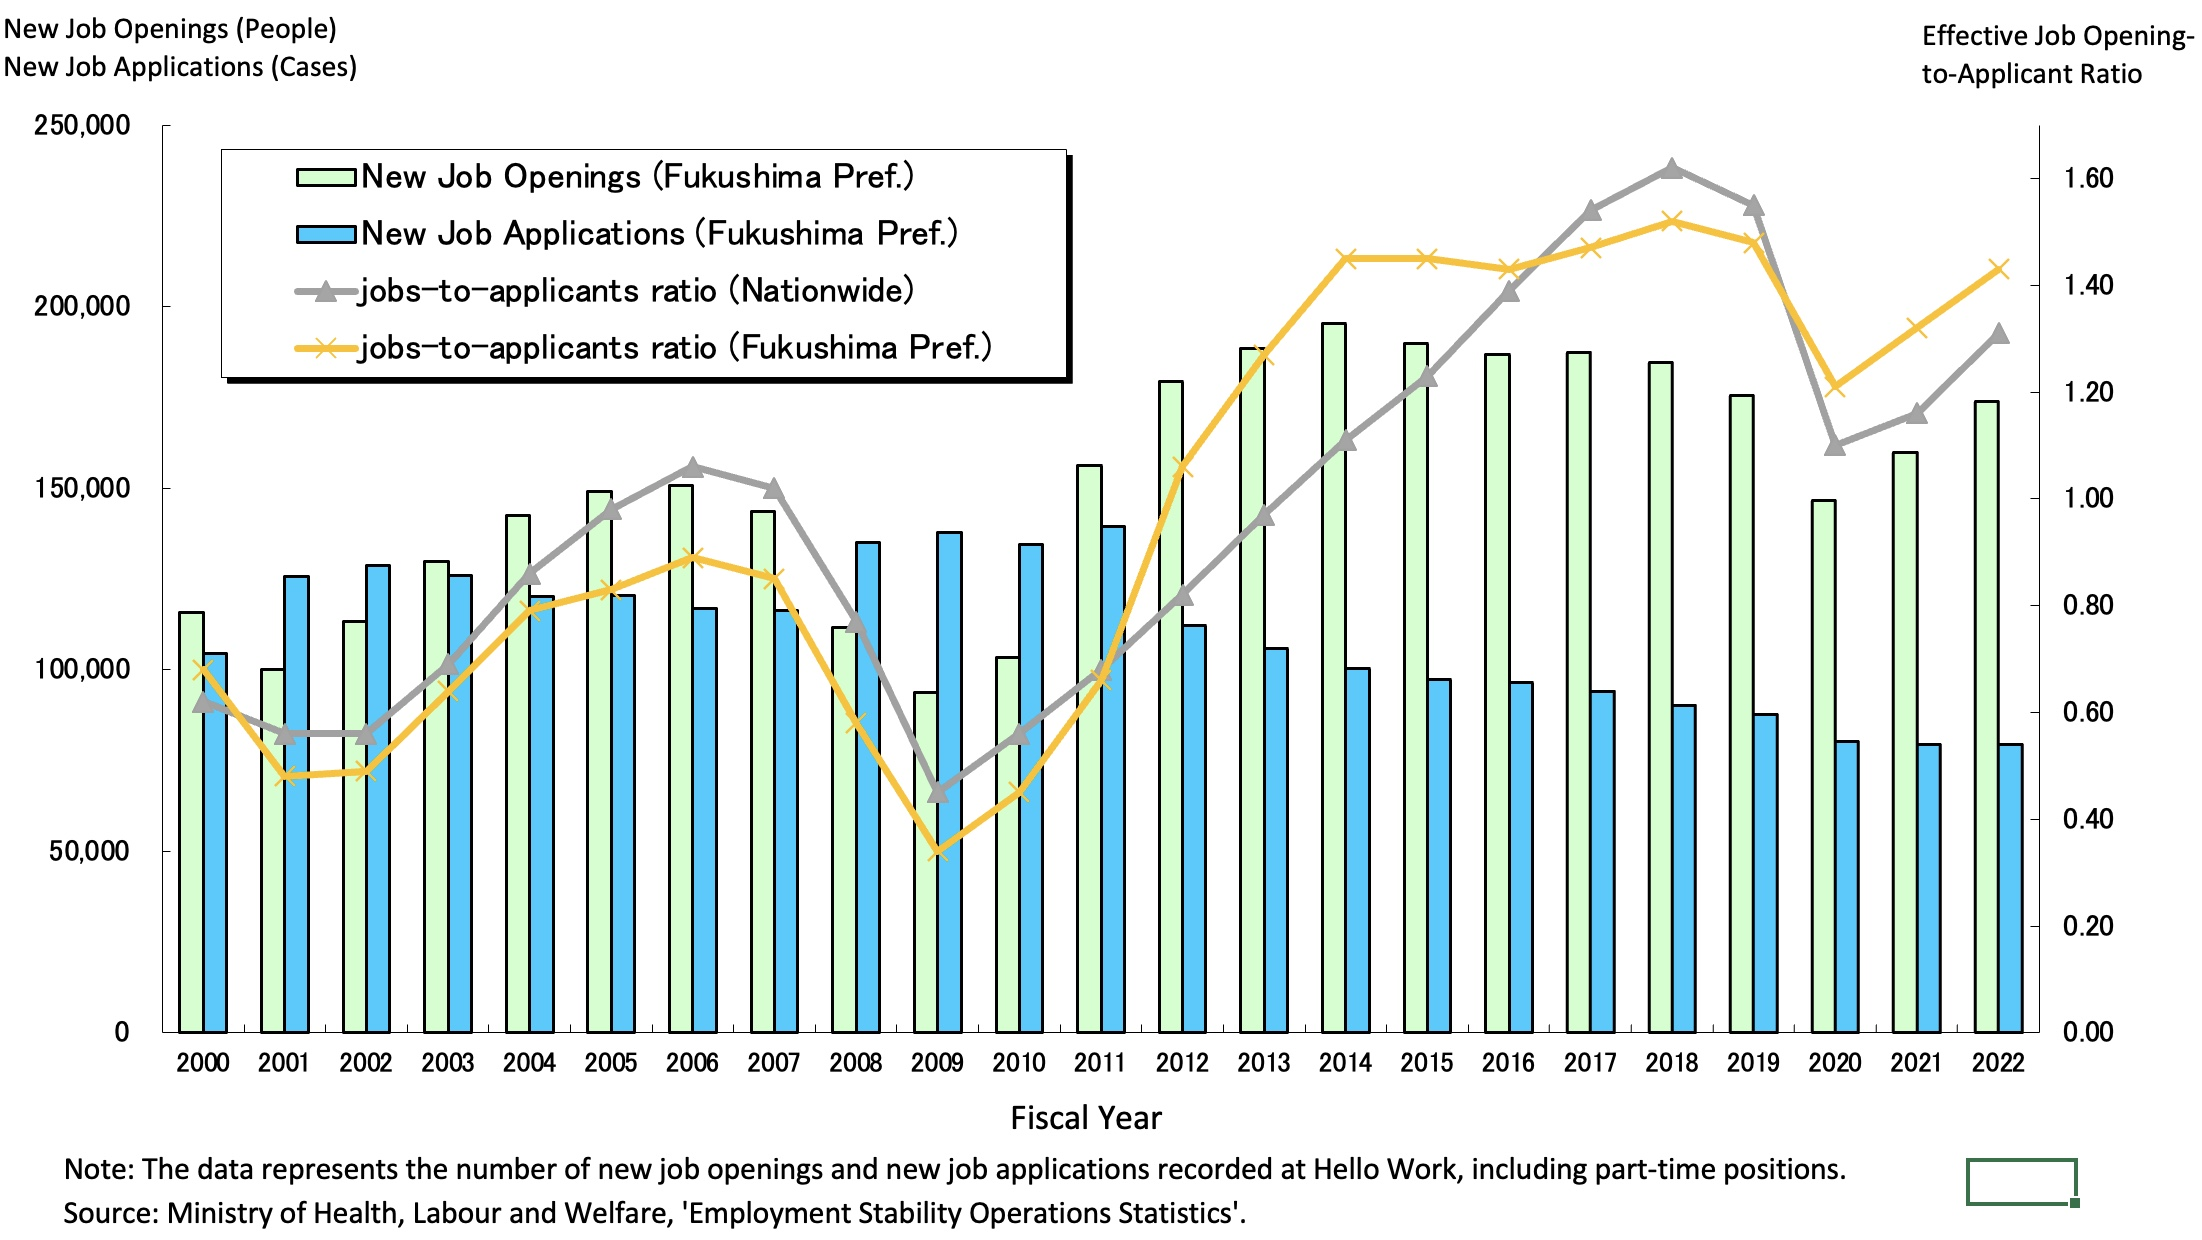
\includegraphics[width=0.9\textwidth]{New Job Openings.jpeg}  % 幅を本文の80%に設定
    \caption{Hello Work Job Openings and Applicants in Fukushima Pref.}
    \label{fig:new_job_openings}
\end{figure}


%Although the number of job openings in the three disaster-affected prefectures of Iwate, Miyagi, and Fukushima initially decreased significantly immediately after the disaster, they have since outperformed the national average. This improvement is largely attributed to the reconstruction demand, including a surge in the construction industry. The first research question of this study investigates how the gender employment gap has evolved under such circumstances.

Figure~\ref{fig:fukushima_Women_ratio_on_applicant} shows a long-term trend of the proportion of women job seekers among total new job applications submitted to Hello Work in Fukushima Prefecture. A higher proportion suggests a narrowing gender employment gap. 

\begin{figure}[h!]
    \centering
    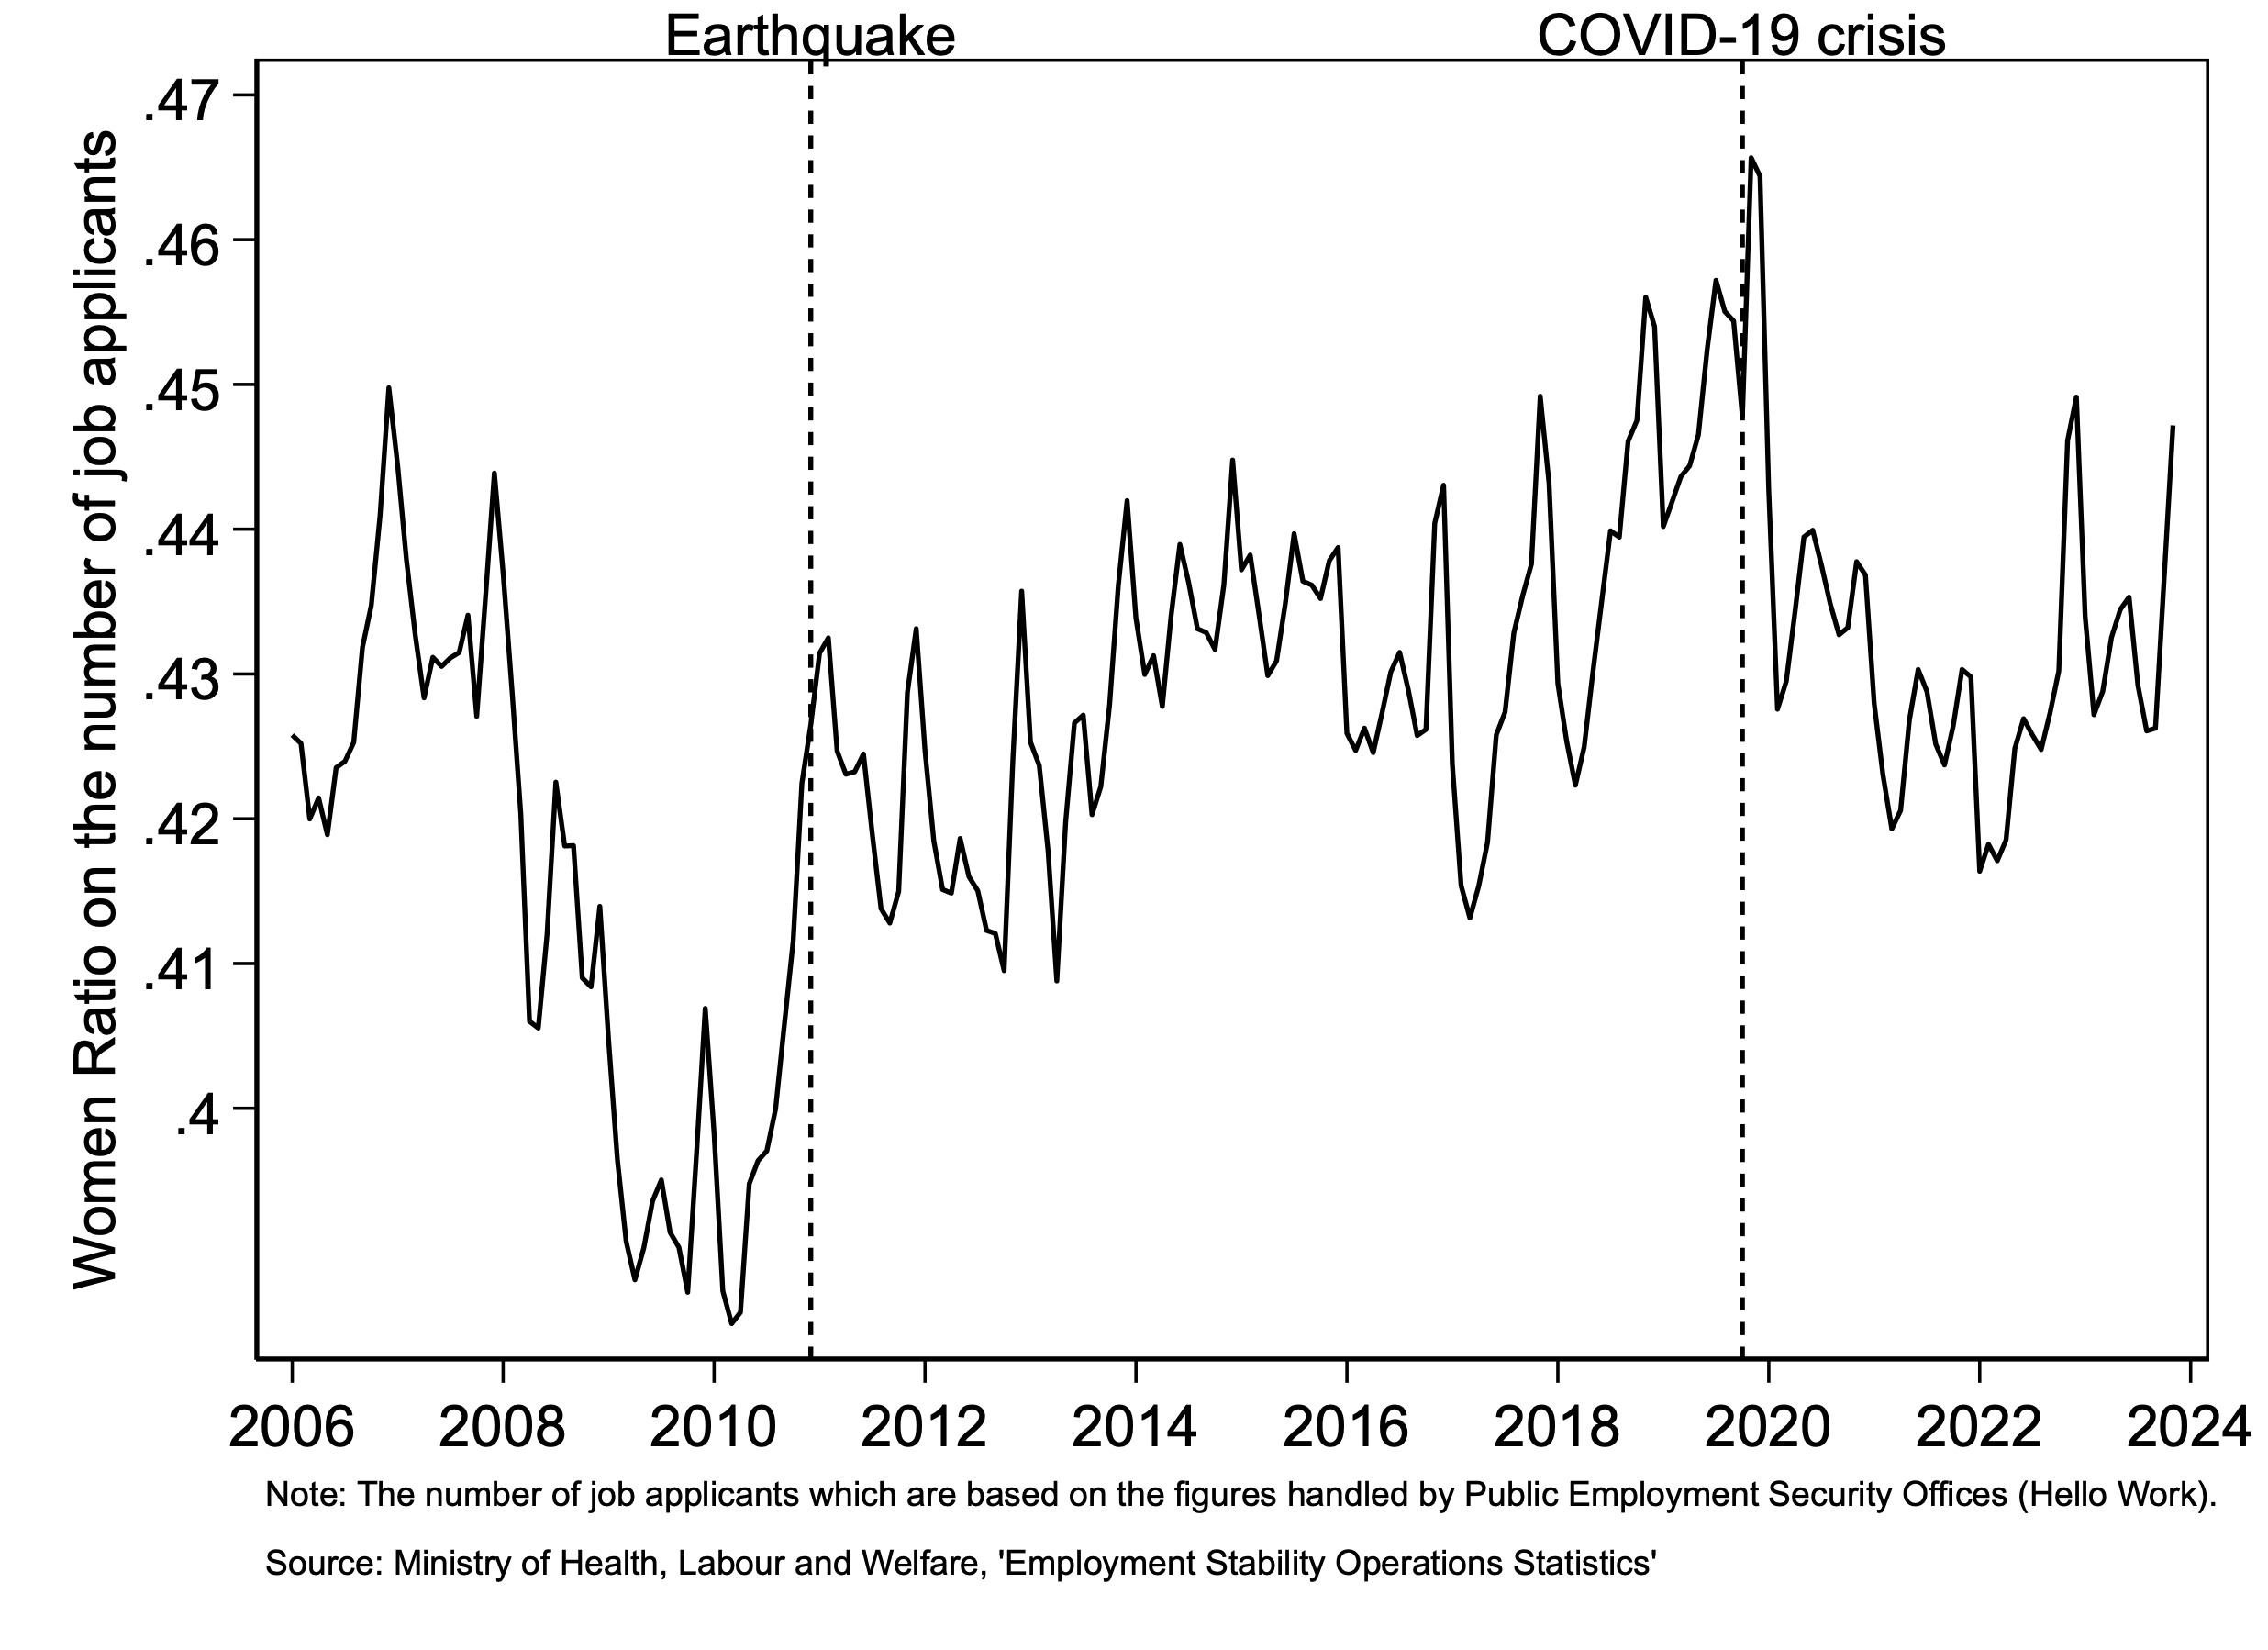
\includegraphics[width=0.9\textwidth]{Women ratio on the number of job applicants.jpg}  % 幅を本文の80%に設定
    \caption{Women ratio on the number of applicants in Fukushima Pref.}
    \label{fig:fukushima_Women_ratio_on_applicant}
\end{figure}

\newpage

The graph reveals that in Fukushima Prefecture, prior to the disaster, from 2008 to the earthquake, the proportion of male job seekers had increased due to the impact of the Lehman Shock. However, post-disaster, there has been a gradual increase in the proportion of female job seekers. In the disaster-affected areas, there is a potential long-term trend of increasing female labor force participation.

Figure~\ref{fig:women_ratio_fukushima} presents a time-series graph showing the proportion of active women job seekers among total job applications submitted to Hello Work in Fukushima Prefecture. Labor market trends in Fukushima Prefecture over the past two decades reveal three distinct phases. During the 2008-2010 global financial crisis, the proportion of female job seekers decreased, suggesting a greater impact on male employment. Following the 2011 Great East Japan Earthquake, there was a sustained increase in the proportion of female job seekers, a trend that persisted throughout the post-disaster period. Since 2020, the COVID-19 pandemic has resulted in a slight decline in the female share of job seekers, potentially indicating a shift in labor market dynamics.


\begin{figure}[h!]
    \centering
    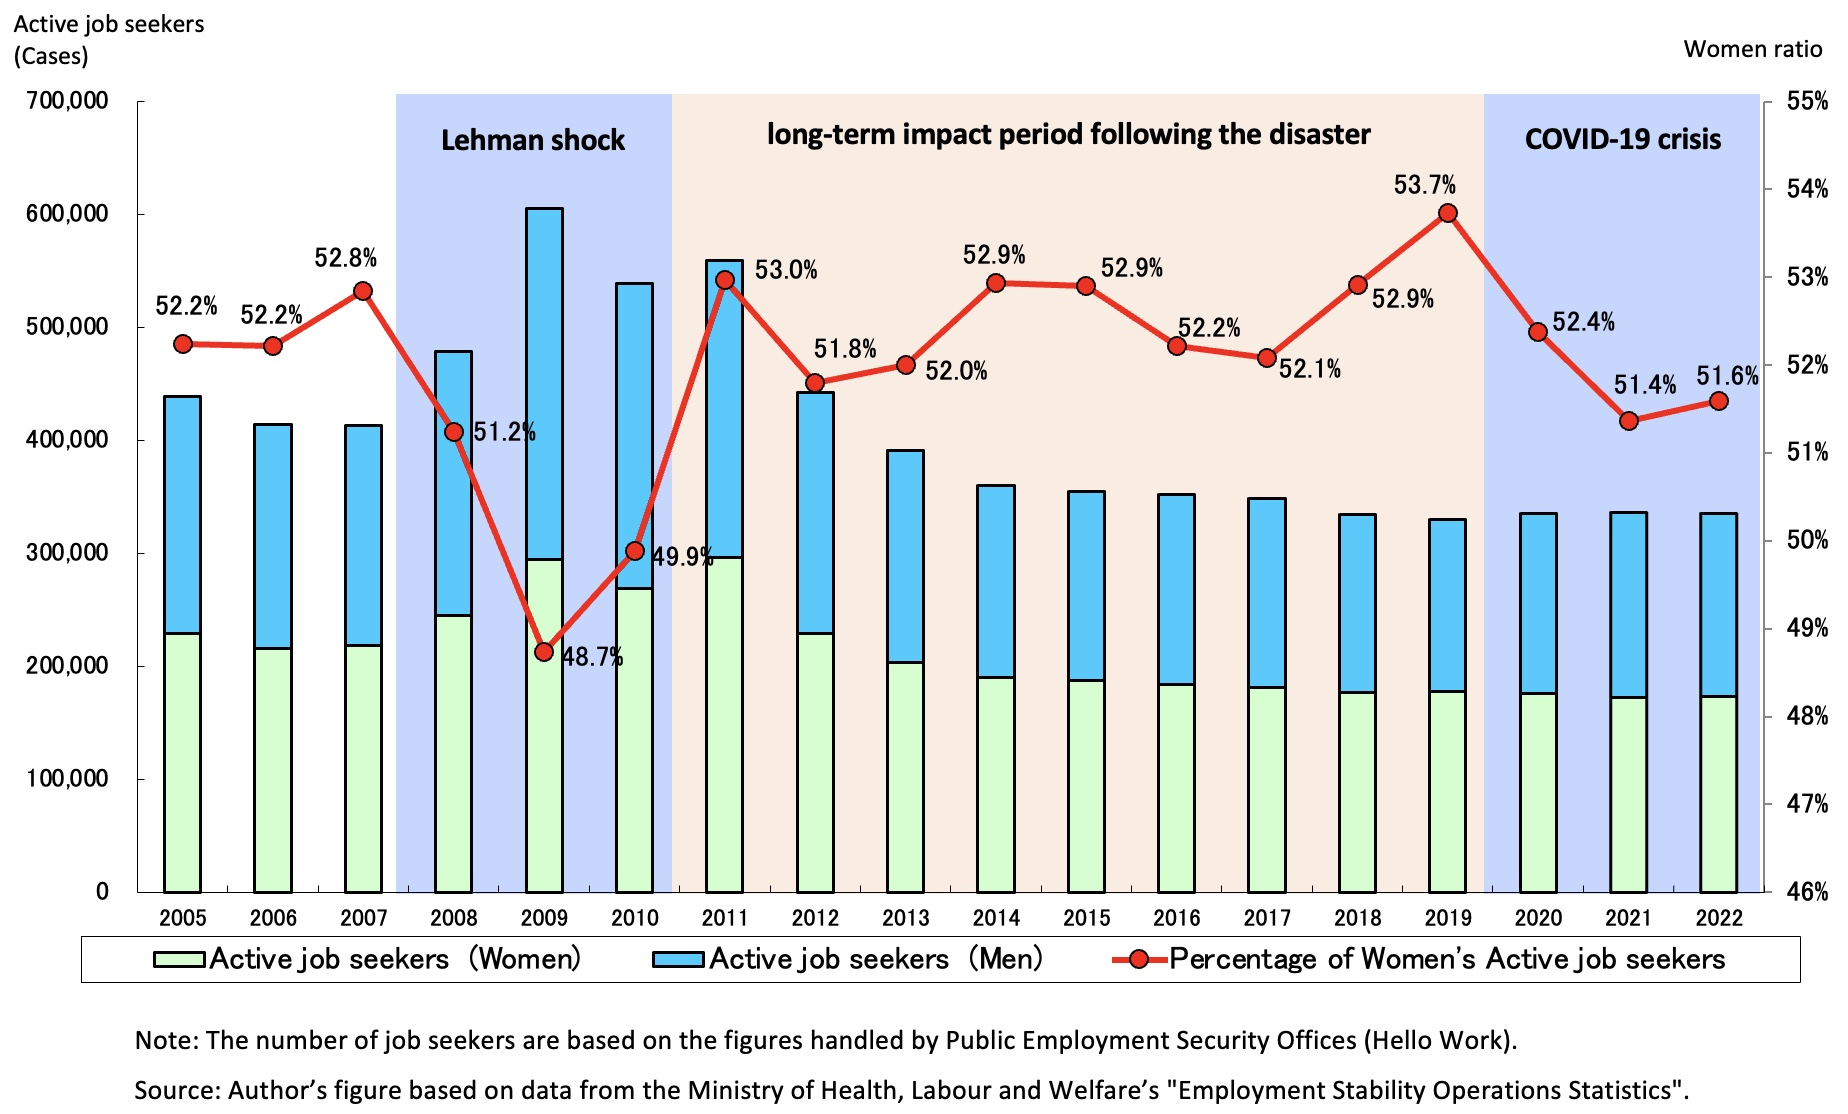
\includegraphics[width=0.9\textwidth]{Women ratio on the number of active job seekers2}  % 幅を本文の80%に設定
    \caption{Women ratio on the number of active job seekers in Fukushima Pref.}
    \label{fig:women_ratio_fukushima}
\end{figure}

\clearpage

Figure~\ref{fig:women_ratio_fukushima2} illustrates both short-term (upper graph) and long-term (lower graph) changes in unemployment insurance recipients in Fukushima Prefecture following the Earthquake. Regarding short-term effects, while overall recipient numbers spiked briefly before returning to pre-disaster levels within a year, the proportion of female recipients also showed a notable increase. This percentage rose from 52-53\% pre-disaster to a peak of 57.2\% in August 2011, five months post-earthquake, before gradually declining. Notably, this peak was 1.7 percentage points higher than the nationwide figure. This trend aligns with reports of heightened short-term employment challenges for women, particularly in heavily impacted coastal areas where female-dominated industries like seafood processing, which employed many part-time women workers, suffered significant damage. Conversely, long-term effects reveal a contrasting trend, with the proportion of female recipients in Fukushima declining relative to the national average. This disparity reached its maximum in 2017, with Fukushima's 55.4\% being 4.7 percentage points lower than the nationwide figure of 60.1\%.


\begin{figure}[h!]
    \centering
    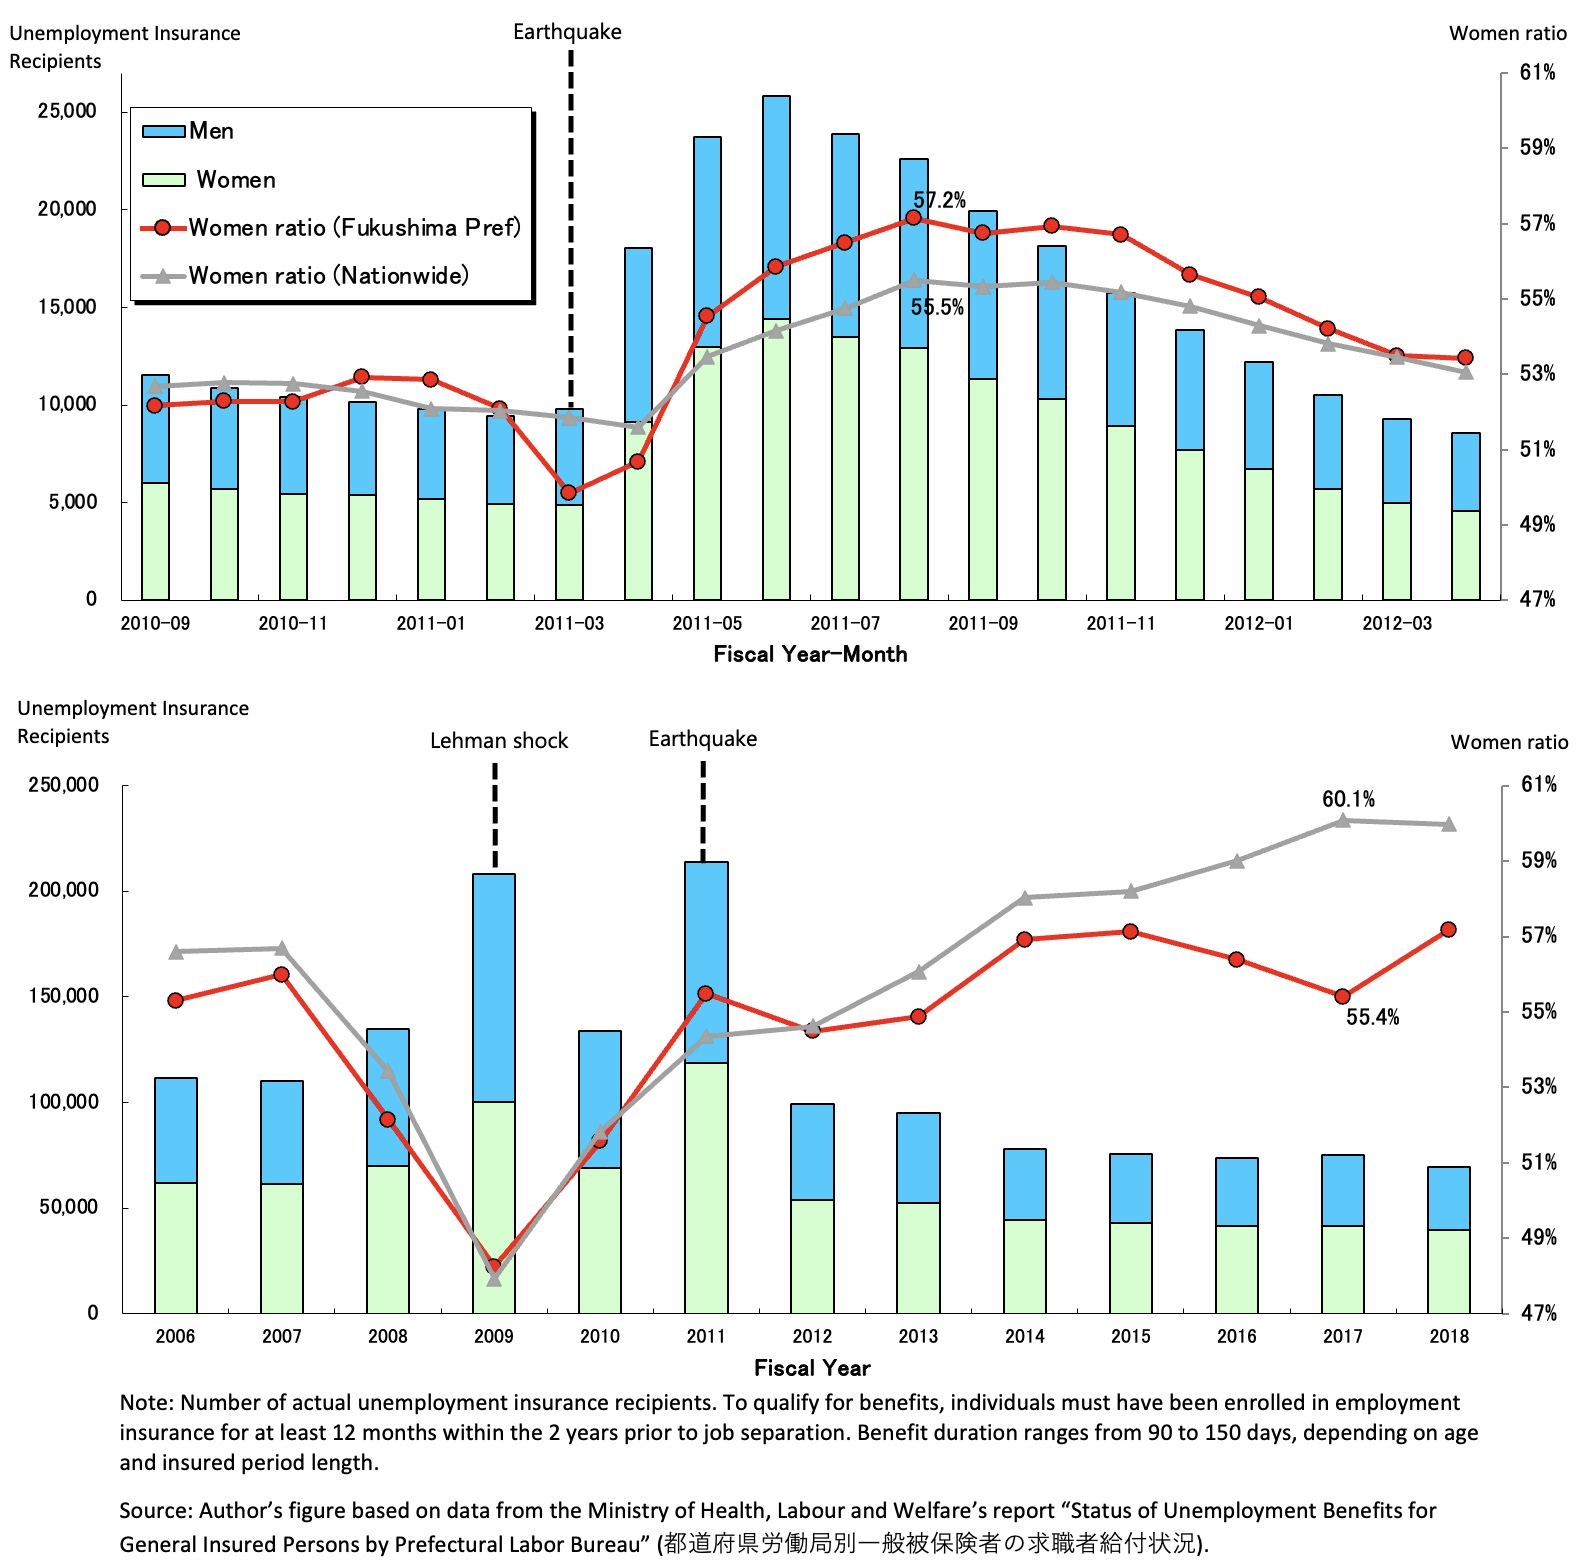
\includegraphics[width=0.9\textwidth]{Number of Actual Unemployment Insurance Recipients2.jpeg}  % 幅を本文の80%に設定
    \caption{Women ratio on the number of Unemployment Insurance Recipients in Fukushima Pref.}
    \label{fig:women_ratio_fukushima2}
\end{figure}


Figure~\ref{fig:employment_insurance_decisions} presents a line graph illustrating the number of unemployment insurance decisions in Fukushima Prefecture, along with the proportion of female applicants relative to total applicants. The graph also includes the national average for comparison. From this graph, it is evident that in Fukushima Prefecture, the proportion of female applicants for unemployment insurance has shown a declining trend post-disaster. This suggests a potential improvement in the labor market conditions for female workers in the disaster-affected areas over the longer term.



\begin{figure}[h!]
    \centering
    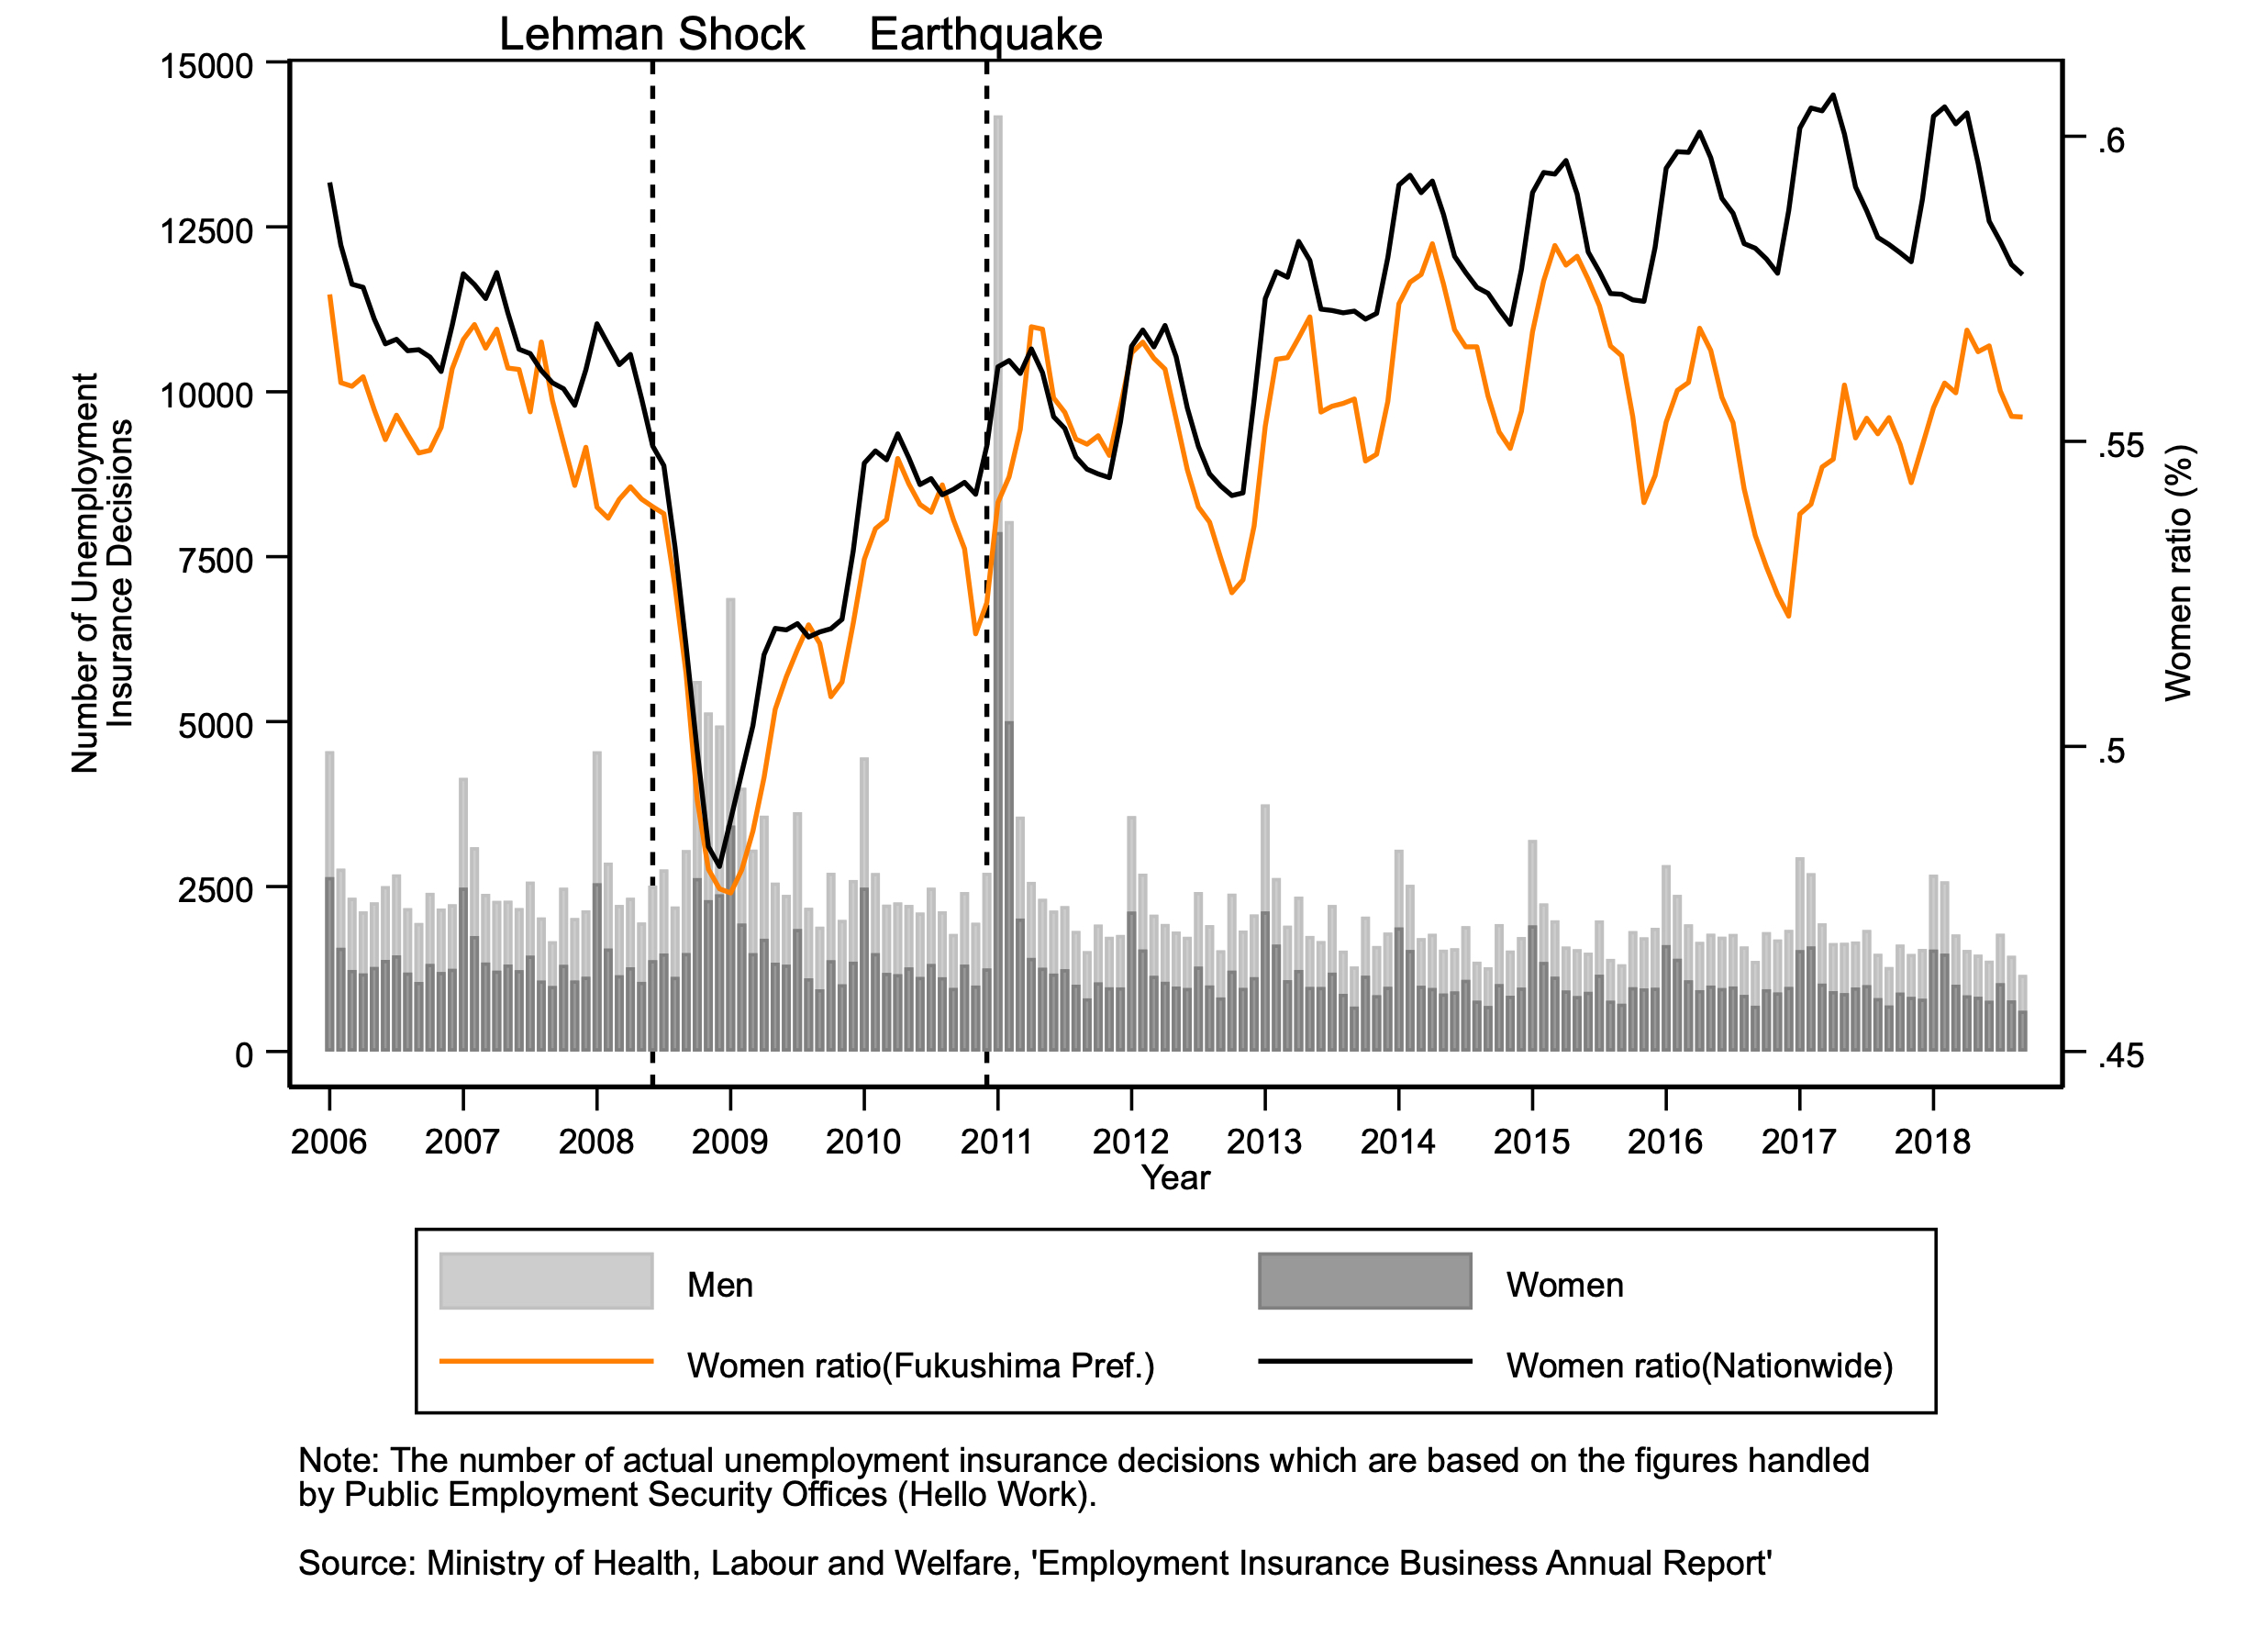
\includegraphics[width=0.9\textwidth]{Number of Unemployment Insurance decisions.jpg}  % 幅を本文の80%に設定
    \caption{Number of Unemployment Insurance Decisions by Gender in Fukushima Pref.}
    \label{fig:employment_insurance_decisions}
\end{figure}


\clearpage
\subsection{Microdata sets analysis}
\label{sec5.1}

To elucidate the causal relationship and mechanisms through which the Great East Japan Earthquake affected the Gender Employment Gap in the disaster-affected regions, this study emphasizes the necessity of analyzing not only regional-level economic statistical panel data but also individual-level microdata pertaining to various socio-economic attributes.

\begin{table}[h!]
    \centering
    \caption{Anonymous individual-level microdata sets}
    \label{tab:list}
    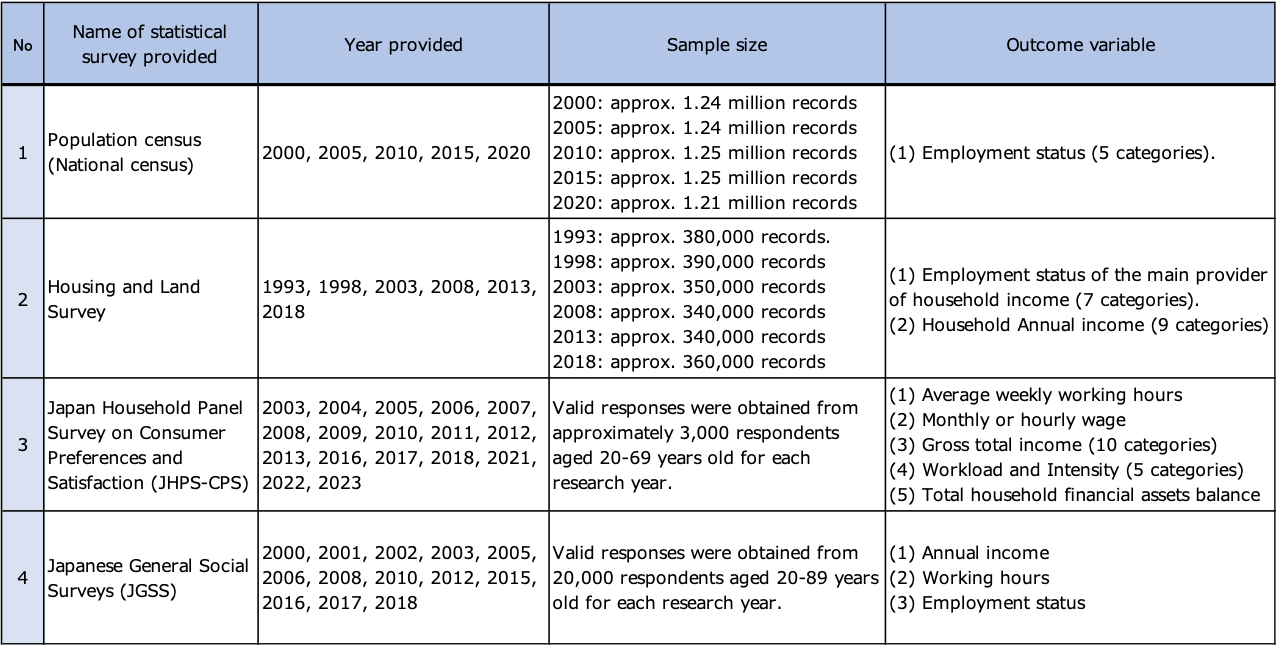
\includegraphics[width=1.0\textwidth]{list.png} 

    \begin{tablenotes}
        \item{\small{\textit{Note}: 'Population census' and 'Housing and Land Survey' were provided by National Statistics Center. JHPS-CPS was provided by Institute of Social and Economic Research, Osaka University. JGSS was provided by JGSS Research Center at Osaka University of Commerce.}}
    \end{tablenotes}
    
\end{table}


\subsection{Empirical model}
\label{sec5.1}

This study statistically estimates whether trends similar to those observed at the regional level in microdata can be identified using four anonymized individual-level datasets: the Japan General Social Survey (JGSS), the Open Survey Data Japan Household Panel Survey on Consumer Preferences and Satisfaction (JHPS-CPS), the National Census, and the Housing and Land Survey. The analysis employs a Difference-in-Differences (DID) approach with Fukushima Prefecture as the Treatment group and other prefectures as the Control group.

The empirical strategy of this study employs DID methodology. For the implementation of DID analysis, I employ a pooled DiD methodology, which is particularly suitable for non-continuous time series data, such as quinquennial census surveys. This approach involves aggregating data into two distinct periods: pre-earthquake and post-earthquake. In cases where continuous annual data is unavailable, this method allows for the bifurcation of the dataset into these two critical temporal segments. By doing so, I can estimate the average treatment effect across the aggregated pre-treatment and post-treatment periods, effectively capturing the impact of the seismic event despite the temporal gaps in data collection. This strategy is especially advantageous when dealing with infrequently collected cross-sectional data, as it maximizes the utilization of available information while adhering to the fundamental principles of DiD analysis.

The model is specified as follows:

\begin{equation}
Y_{ipt} = \alpha_{p} + \beta D_{p} + \eta Post_{t} + \gamma (D_{pt} * Post_{t}) + X_{ipt} + \epsilon_{ipt}
\end{equation}

Here, \( Y_{idt} \) denotes the outcome variable, such as the employment rate, annual income, or working hours, for individual \( i \) in prefecture \( p \) at year \( t \). \( \gamma \) represents the disasters effect that I aim to estimate. 

\begin{equation}
\begin{aligned}
E[\text{DiD estimator}] \\
&= (E[Y_{ipt}|D_i = 1, \text{Post}_t = 1] - E[Y_{ipt}|D_i = 1, \text{Post}_t = 0]) \\
&- (E[Y_{ipt}|D_i = 0, \text{Post}_t = 1] - E[Y_{ipt}|D_i = 0, \text{Post}_t = 0]) \\
&= (\alpha_{p} + \beta + \eta + \gamma - \beta_0 - \beta) - (\alpha_{p} + \eta - \alpha_{p}) \\
&= \gamma
\end{aligned}
\end{equation}


ーーーーーーーーーーーーー

To adequately capture the dynamic effects of natural disasters, which inherently have long-term and evolving impacts, I employ a Two-Way Fixed Effects Event Study (TWFE Event Study) approach. This method extends the traditional Difference-in-Differences (DiD) framework to account for the temporal dimension of disaster impacts. The model is specified as follows:

\begin{equation}
Y_{ipt} = \beta_ip + \eta_t + \sum_{l}^{} \gamma_l 1 [t-s_{pt} = l] + \epsilon_{ipt}
\end{equation}

Where: \\
$Y_{ipt}$ is the outcome variable for individual \( i \) in prefecture \( p \) at year \( t \) \\
$\beta_ip$ represents unit fixed effects for individual \( i \) in prefecture \( p \) \\
$\eta_t$ denotes time fixed effects \\
$s_{i}$ is the timing of the earthquake occurrence \\
$l$ is the number of periods relative to the earthquake
$\gamma_l$ captures the effect of the disaster $l$ periods after (or before) its occurrence \\
$\epsilon_{ipt}$ is the error term

This specification allows for estimating the dynamic treatment effects over an extended period, both pre- and post-disaster, thereby providing a comprehensive understanding of the disaster's evolving impact on economic outcomes.

ーーーーーーーーーーーーー

In the Microdata sets analysis chapter, using individual-level data from the Japanese General Social Surveys (JGSS), I investigate changes in individual annual income by gender between the three disaster-affected prefectures and other prefectures before and after the earthquake. 

The pre/post income band difference for affected prefecture women was statistically significant (Table 3; T-value: -1.849, P-value: 0.065). As Figure~\ref{fig:Kernel_density} and Table~\ref{table:mean_of_annual_income} shows, only this ‘Women in affected prefectures’ group's average income bands shifted right (increased) pre/post-disaster.

\begin{figure}[h!]
    \centering
    \includegraphics[width=0.9\textwidth]{Kernel density graphs of respondent’s annual income from main job.png}  % 幅を本文の80%に設定
    \caption{Kernel density graphs of respondent’s annual income from main job (Income bands, N= 20,119)}
    \label{fig:Kernel_density}
\end{figure}


\begin{table}[h!]
    \centering
    \caption{Mean of annual income: Pre/Post-disaster period (Income bands, N=20,119)}
    \label{tab:annual_income}
    
\includegraphics[width=0.9\textwidth]{Annual income table.png}  % 幅を本文の80%に設定
    \label{table:mean_of_annual_income}
\end{table}

\newpage

\section{Discussion}
\label{sec5}

\subsection{Conceptual framework}
\label{sec5.1}

The exact magnitude of natural disaster's impacts on output is widely debated. The case of the Great East Japan Earthquake illustrates the complexity of the reconstruction process and rational household responses when communities are disrupted by the disasters. Figure~\ref{fig:conceptual_model} presents changes in female worker's income in a disaster-affected prefecture overtime as a conceptual framework for understanding overall effect. $T0$ represents the time point when the earthquake occurred. 

At Phase 1, according to the Risk Adjustment Hypothesis, an exogenous shock would alter the production function of both sellers and buyers, disproportionately affecting female employment due to the higher prevalence of non-regular workers among women.

At Phase 2, the female employment recovery rate would surpass that of males, driven by three factors: the post-disaster spike in reconstruction booming, household shock coping strategies necessitating women to seek higher payment jobs, and government policies aimed at promoting employment opportunities for groups vulnerable to disasters.

At Phase 3, in the long term, the impact of the disaster gradually diminishes, and the income levels of women in the affected areas converge towards the normal.


\begin{figure}[h!]
    \centering
    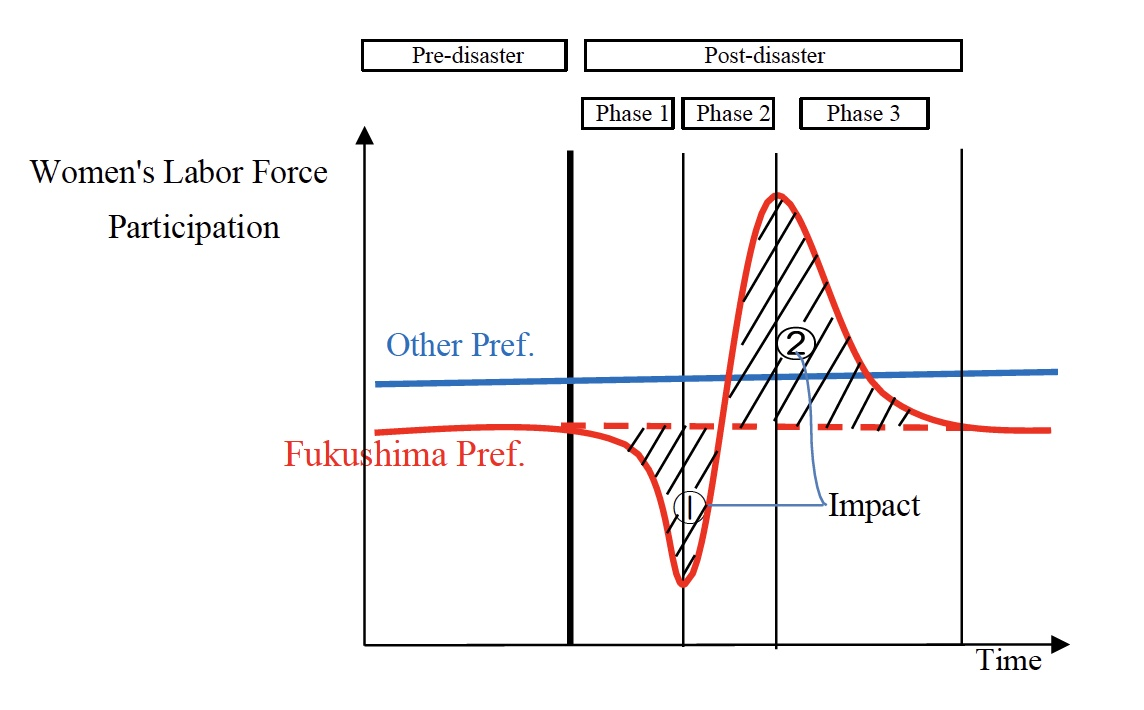
\includegraphics[width=0.9\textwidth]{A conceptual model.jpeg}  % 幅を本文の80%に設定
    \caption{A conceptual framework for understanding overall disaster's effect on income}
    \label{fig:conceptual_model}
\end{figure}


Initially, these events disproportionately impacted female workers negatively. However, the earthquake and nuclear disaster potentially accelerated women's labor market participation by fundamentally disrupting communities bound by traditional gender roles. In the short term, the disaster and nuclear accident had a more severe negative impact on female workers. However, in the long term, this catastrophic event, while devastating, may have inadvertently challenged long-standing societal norms, thus facilitating increased female workforce engagement. The conceptual framework for considering gender dynamics and disaster impacts adapted the below basic model which captures the change in female worker's income overtime, measuring its cumulative effect:

\begin{equation}
\int_{T0}^{T2} [YF_F(t) - YF_C(t)] dt
\end{equation}

where $YF_F(t)$ represents the female worker's income in Fukushima Prefecture at time $t$, and $YF_C(t)$ represents the counterfactual which assumes the earthquake did not occur, assuming the parallel trend of control prefectures. $T2$ denotes the end of the impact period (the end of Phase 3).

In this model, the present value of the disaster's impact on female worker's income is captured by the integral. The result of the integration corresponds to the area of the hatched sections (\ding{172}+\ding{173}) in the graph, representing the sum of negative effects during the immediate post-disaster period and positive effects during the disaster recovery period.

For a more detailed analysis, the model can be decomposed as follows:

\begin{equation}
\int_{T0}^{T1} [YF_F(t) - YF_C(t)] dt + \int_{T1}^{T2} [YF_F(t) - YF_C(t)] dt
\end{equation}

where $T1$ represents the point in time at which the actual female worker's income line intersects with the counterfactual line, depicted by the red dashed line in the graph. This equation allows for separate calculation of the negative impact (\ding{172}) and the positive impact (\ding{173}), while still computing their sum.

Utilizing this model enables the quantification of the overall impact of the disaster on female worker's income, facilitating an analysis that considers both the negative shock in the immediate post-disaster period and the subsequent growth during the disaster recovery phase. This approach provides a comprehensive framework for evaluating the dynamic effects of disasters on gender-specific impacts in affected prefecture.


\subsection{Household decision model}
\label{sec5.1}

This study models how households made economically rational decisions following the Great East Japan Earthquake by utilizing a microdata-based DID analysis, which supports the gender gaps identified in regional-level statistical data. This household model suggests that the destruction of communities by the earthquake also disrupted traditional gender norms and local gift economies, potentially forcing women into the labor market to get higher income.

This study constructs a household decision-making model to elucidate the fluctuations in female employment before and after a major earthquake. The model draws upon the agricultural household model framework (Huffman \& El-Osta, 1997; Omamo, 1998; Key, Sadoulet, \& Janvry, 2000), adapting it to the context of disaster-affected urban and rural areas. It incorporates elements from development economics, which suggest an increase in household members' labour supply for higher payment jobs as a shock-coping strategy.
The model delineates three distinct phases: the immediate aftermath, the recovery period, and the long-term equilibrium. In Phase 1, it accounts for the exogenous shock's impact on production functions and the disproportionate effect on female employment due to the prevalence of non-regular work among women. Phase 2 captures the interplay between reconstruction booming, household coping strategies necessitating higher income, and government policies promoting women's work opportunities. Finally, Phase 3 models the gradual convergence of female income levels in affected areas towards the national average as the disaster's impact wanes over time.
By integrating these elements, the model aims to provide a comprehensive framework for analyzing the dynamics of female worker's income and intra-household bargaining power in the wake of a major natural disaster.


% すべての文献を引用リストに追加
\nocite{*}

% 参考文献リストの場所を示す
\bibliography{references}  % 'references.bib'ファイルの名前を指定
\bibliographystyle{plain}  % 引用スタイルを指定


\end{document}
